\documentclass[]{book}
\usepackage{lmodern}
\usepackage{amssymb,amsmath}
\usepackage{ifxetex,ifluatex}
\usepackage{fixltx2e} % provides \textsubscript
\ifnum 0\ifxetex 1\fi\ifluatex 1\fi=0 % if pdftex
  \usepackage[T1]{fontenc}
  \usepackage[utf8]{inputenc}
\else % if luatex or xelatex
  \ifxetex
    \usepackage{mathspec}
  \else
    \usepackage{fontspec}
  \fi
  \defaultfontfeatures{Ligatures=TeX,Scale=MatchLowercase}
\fi
% use upquote if available, for straight quotes in verbatim environments
\IfFileExists{upquote.sty}{\usepackage{upquote}}{}
% use microtype if available
\IfFileExists{microtype.sty}{%
\usepackage{microtype}
\UseMicrotypeSet[protrusion]{basicmath} % disable protrusion for tt fonts
}{}
\usepackage[margin=1in]{geometry}
\usepackage{hyperref}
\hypersetup{unicode=true,
            pdftitle={Patterns and Trends in Environmental Data},
            pdfauthor={Patrick Laube and Nils Ratnaweera},
            pdfborder={0 0 0},
            breaklinks=true}
\urlstyle{same}  % don't use monospace font for urls
\usepackage{color}
\usepackage{fancyvrb}
\newcommand{\VerbBar}{|}
\newcommand{\VERB}{\Verb[commandchars=\\\{\}]}
\DefineVerbatimEnvironment{Highlighting}{Verbatim}{commandchars=\\\{\}}
% Add ',fontsize=\small' for more characters per line
\usepackage{framed}
\definecolor{shadecolor}{RGB}{248,248,248}
\newenvironment{Shaded}{\begin{snugshade}}{\end{snugshade}}
\newcommand{\KeywordTok}[1]{\textcolor[rgb]{0.13,0.29,0.53}{\textbf{#1}}}
\newcommand{\DataTypeTok}[1]{\textcolor[rgb]{0.13,0.29,0.53}{#1}}
\newcommand{\DecValTok}[1]{\textcolor[rgb]{0.00,0.00,0.81}{#1}}
\newcommand{\BaseNTok}[1]{\textcolor[rgb]{0.00,0.00,0.81}{#1}}
\newcommand{\FloatTok}[1]{\textcolor[rgb]{0.00,0.00,0.81}{#1}}
\newcommand{\ConstantTok}[1]{\textcolor[rgb]{0.00,0.00,0.00}{#1}}
\newcommand{\CharTok}[1]{\textcolor[rgb]{0.31,0.60,0.02}{#1}}
\newcommand{\SpecialCharTok}[1]{\textcolor[rgb]{0.00,0.00,0.00}{#1}}
\newcommand{\StringTok}[1]{\textcolor[rgb]{0.31,0.60,0.02}{#1}}
\newcommand{\VerbatimStringTok}[1]{\textcolor[rgb]{0.31,0.60,0.02}{#1}}
\newcommand{\SpecialStringTok}[1]{\textcolor[rgb]{0.31,0.60,0.02}{#1}}
\newcommand{\ImportTok}[1]{#1}
\newcommand{\CommentTok}[1]{\textcolor[rgb]{0.56,0.35,0.01}{\textit{#1}}}
\newcommand{\DocumentationTok}[1]{\textcolor[rgb]{0.56,0.35,0.01}{\textbf{\textit{#1}}}}
\newcommand{\AnnotationTok}[1]{\textcolor[rgb]{0.56,0.35,0.01}{\textbf{\textit{#1}}}}
\newcommand{\CommentVarTok}[1]{\textcolor[rgb]{0.56,0.35,0.01}{\textbf{\textit{#1}}}}
\newcommand{\OtherTok}[1]{\textcolor[rgb]{0.56,0.35,0.01}{#1}}
\newcommand{\FunctionTok}[1]{\textcolor[rgb]{0.00,0.00,0.00}{#1}}
\newcommand{\VariableTok}[1]{\textcolor[rgb]{0.00,0.00,0.00}{#1}}
\newcommand{\ControlFlowTok}[1]{\textcolor[rgb]{0.13,0.29,0.53}{\textbf{#1}}}
\newcommand{\OperatorTok}[1]{\textcolor[rgb]{0.81,0.36,0.00}{\textbf{#1}}}
\newcommand{\BuiltInTok}[1]{#1}
\newcommand{\ExtensionTok}[1]{#1}
\newcommand{\PreprocessorTok}[1]{\textcolor[rgb]{0.56,0.35,0.01}{\textit{#1}}}
\newcommand{\AttributeTok}[1]{\textcolor[rgb]{0.77,0.63,0.00}{#1}}
\newcommand{\RegionMarkerTok}[1]{#1}
\newcommand{\InformationTok}[1]{\textcolor[rgb]{0.56,0.35,0.01}{\textbf{\textit{#1}}}}
\newcommand{\WarningTok}[1]{\textcolor[rgb]{0.56,0.35,0.01}{\textbf{\textit{#1}}}}
\newcommand{\AlertTok}[1]{\textcolor[rgb]{0.94,0.16,0.16}{#1}}
\newcommand{\ErrorTok}[1]{\textcolor[rgb]{0.64,0.00,0.00}{\textbf{#1}}}
\newcommand{\NormalTok}[1]{#1}
\usepackage{longtable,booktabs}
\usepackage{graphicx,grffile}
\makeatletter
\def\maxwidth{\ifdim\Gin@nat@width>\linewidth\linewidth\else\Gin@nat@width\fi}
\def\maxheight{\ifdim\Gin@nat@height>\textheight\textheight\else\Gin@nat@height\fi}
\makeatother
% Scale images if necessary, so that they will not overflow the page
% margins by default, and it is still possible to overwrite the defaults
% using explicit options in \includegraphics[width, height, ...]{}
\setkeys{Gin}{width=\maxwidth,height=\maxheight,keepaspectratio}
\IfFileExists{parskip.sty}{%
\usepackage{parskip}
}{% else
\setlength{\parindent}{0pt}
\setlength{\parskip}{6pt plus 2pt minus 1pt}
}
\setlength{\emergencystretch}{3em}  % prevent overfull lines
\providecommand{\tightlist}{%
  \setlength{\itemsep}{0pt}\setlength{\parskip}{0pt}}
\setcounter{secnumdepth}{5}
% Redefines (sub)paragraphs to behave more like sections
\ifx\paragraph\undefined\else
\let\oldparagraph\paragraph
\renewcommand{\paragraph}[1]{\oldparagraph{#1}\mbox{}}
\fi
\ifx\subparagraph\undefined\else
\let\oldsubparagraph\subparagraph
\renewcommand{\subparagraph}[1]{\oldsubparagraph{#1}\mbox{}}
\fi

%%% Use protect on footnotes to avoid problems with footnotes in titles
\let\rmarkdownfootnote\footnote%
\def\footnote{\protect\rmarkdownfootnote}

%%% Change title format to be more compact
\usepackage{titling}

% Create subtitle command for use in maketitle
\newcommand{\subtitle}[1]{
  \posttitle{
    \begin{center}\large#1\end{center}
    }
}

\setlength{\droptitle}{-2em}

  \title{Patterns and Trends in Environmental Data}
    \pretitle{\vspace{\droptitle}\centering\huge}
  \posttitle{\par}
  \subtitle{Master ENR, Spring Semester 2019}
  \author{Patrick Laube and Nils Ratnaweera}
    \preauthor{\centering\large\emph}
  \postauthor{\par}
      \predate{\centering\large\emph}
  \postdate{\par}
    \date{02 May, 2019}


\begin{document}
\maketitle

{
\setcounter{tocdepth}{1}
\tableofcontents
}
\chapter*{Introduction Chapter}\label{introduction-chapter}
\addcontentsline{toc}{chapter}{Introduction Chapter}

For our practical \texttt{R} course building-up skills for analyzing
movement data in the software environment \texttt{R}, you'll be using
data from the ZHAW project
\href{https://www.zhaw.ch/de/lsfm/institute-zentren/iunr/integrative-oekologie/wildtiermanagement/referenzprojekte/}{``Prävention
von Wildschweinschäden in der Landwirtschaft''}.

The project investigates the spatiotemporal movement patterns of wild
boar (\emph{Sus scrofa}) in agricultural landscapes. We will study the
trajectories of these wild boar, practicing the most basic analysis
tasks of Computational Movement Analysis (CMA).

\textbf{Please note:} we are given application data from an ongoing
research project. Capturing wild living animals and then equipping them
with GPS collars is a very labor and cost intensive form of research.
Consequently, data resulting such campaigns is a very valuable asset
that must be protected. So, please do not pass on this data, for any use
beyond this module contact Patrick Laube or the data owner Stefan Suter
(\href{mailto:suts@zhaw.ch}{\nolinkurl{suts@zhaw.ch}}).

\chapter{Exercise 1}\label{exercise-1}

Exercise 1 covers the necessary steps for getting ready in \texttt{R}
and some basic concepts for setting up a well-structured \texttt{R}
project. The lesson introduces how additional packages that provide
useful functions for data science are made available and how spatial
data is handled. The exercise concludes with the creation of your first
map featuring movement data.

\section{Leaning outcomes}\label{leaning-outcomes}

\begin{itemize}
\tightlist
\item
  You learn how to structure an \texttt{R} project.
\item
  You can read movement data from a .csv-file into a \texttt{data.frame}
\item
  You can convert spatial point data from a \texttt{data.frame} to a
  spatial object \texttt{sf}
\item
  You can perform basic spatial operations on spatial objects in
  \texttt{R}
\item
  You can produce simple maps of your spatial data using
  \texttt{ggplot2}
\item
  You can produce simple maps of your spatial data using \texttt{tmap}
\end{itemize}

\section{Prerequisites}\label{prerequisites}

Readings Skills from ``R for Data Science'' (Wickham and Grolemund
\protect\hyperlink{ref-wickham2017}{2017}):

\begin{itemize}
\tightlist
\item
  RS1.1 Preface (16p, ix-xxiv)
\item
  RS1.2 Chap2 Workflow basics (3p, 37-39)
\item
  RS1.3 Chap4 Workflow scripts (3p, 77-79)
\item
  RS1.4 Chap6 workflow projects (6p, 111-116)
\item
  RS1.5 Chap8 Data Import with \texttt{readr} (21p)
\item
  RS1.6 Chap13 Date and Times with \texttt{lubridate} (18p, 237-256)
\end{itemize}

\section{Preperation}\label{preperation}

If you haven't already, install the packages \texttt{tidyverse}, and
\texttt{devtools} (using \texttt{install.packages()}). Additionally,
install the packages \texttt{sf}, \texttt{raster} and
\texttt{ggspatial}. \textbf{Restart your \texttt{R} session after
installing all these packages.}

\begin{Shaded}
\begin{Highlighting}[]
\KeywordTok{install.packages}\NormalTok{(}\StringTok{"tidyverse"}\NormalTok{)}
\KeywordTok{install.packages}\NormalTok{(}\StringTok{"sf"}\NormalTok{)}
\KeywordTok{install.packages}\NormalTok{(}\StringTok{"raster"}\NormalTok{)}
\end{Highlighting}
\end{Shaded}

\section{Tasks and inputs}\label{tasks-and-inputs}

\subsection{Task 1: Initialize project}\label{task-1-initialize-project}

Create a new \emph{RStudio Project}. As recommended in Wickham and
Grolemund (\protect\hyperlink{ref-wickham2017}{2017}), remove the option
``\emph{Restore .RData into workspace at startup}'' and set the option
``\emph{save workspace to .RData on exit}'' to ``\emph{Never}''.

Create a new .R (or .Rmd) File and divide it into the sections necessary
in a classical Data Science Workflow. In .R Files, ``Sections'' can be
created within RStudio by adding Comments (\texttt{\#}) with at least 4
trailing dashes, equal, or pound signs ( \texttt{-},
\texttt{=},\texttt{\#}). In .Rmd Files, their are created with leading
pound signs (\texttt{\#}).

Sections allow code folding (try clicking on the small triangle next to
the line number) and facilitate navigation (try the shortcut:
\texttt{Shift}+\texttt{Alt}+\texttt{J}). We recommend following
sections:

\begin{itemize}
\tightlist
\item
  Loading environment / libraries
\item
  Data import
\item
  Data cleansing
\item
  Data analysis and visualization
\end{itemize}

\subsection{Task 2: Import data}\label{task-2-import-data}

In section ``data import'', import the file
\texttt{wildschwein\_BE.csv}. Obtain this file from moodle.

Note:

\begin{itemize}
\tightlist
\item
  If your are using
  \href{https://support.rstudio.com/hc/en-us/articles/218611977-Importing-Data-with-RStudio}{a
  graphical tool} to import your code, make sure you save the
  corresponding code in your R Script. This is important in regard to
  the reproducibility of your script and will ensure that your workflow
  is documented without gaps. We'd rather recommend to move away from
  using graphical tools and focus on using code.
\item
  We recommend using one of the \texttt{tidyverse} functions from the
  \texttt{readr} package to import your data (they all begin with
  ``\texttt{read\_*}, note the underscore). These functions are less
  error prone than the base \texttt{R} functions (\texttt{read.*}).
  Specifically for the wild boar data, we recommend
  \texttt{read\_delim()}.
\item
  If you use \texttt{read\_delim()} and receive warnings during import,
  have a look at these warnings by using the function
  \texttt{problems()}. Resolve these problems until import runs without
  warnings.
\item
  Assign correct data types as necessary and make sure the time zone is
  set correctly for the date/time column.
\item
  For everyone working on the RStudio Server: You will first need to
  upload this data to the server using the ``\emph{upload}''-button in
  the ``\emph{Files}'' tab.
\end{itemize}

\subsection{Task 3: Explore Data}\label{task-3-explore-data}

We will use a range of different visualization tools (i.e.~R-packages)
in this course. Several packages techniques have emerged in recent
years, each with their specific strengths and weaknesses. While
\texttt{base::plot()}is quick and simple, it not very scalable with
growing complexity. \texttt{ggplot2} offers solutions for most use cases
and has an elegant, consistent syntax that is easy to get accustomed to.
We will get to know other techniques later in the course.

Get an overview of your data by creating a first ``map-like'' plot of
your data producing a simple scatter plot with \texttt{ggplot2}. Setting
up a \texttt{ggplot} with our data is done using the command
\texttt{ggplot(wildschwein\_BE,\ aes(Long,\ Lat,\ colour\ =\ TierID))}.
Creating a map is done via the basic scatter plot command
\texttt{geom\_point()}. Use \texttt{coord\_map()} to get a reasonable
aspect ratio of \texttt{Lat} and \texttt{Long}. Assigning every
individual its own colour is done using the \texttt{ggplot} argument
\texttt{colour\ =}.

Save your code in the appropriate section.

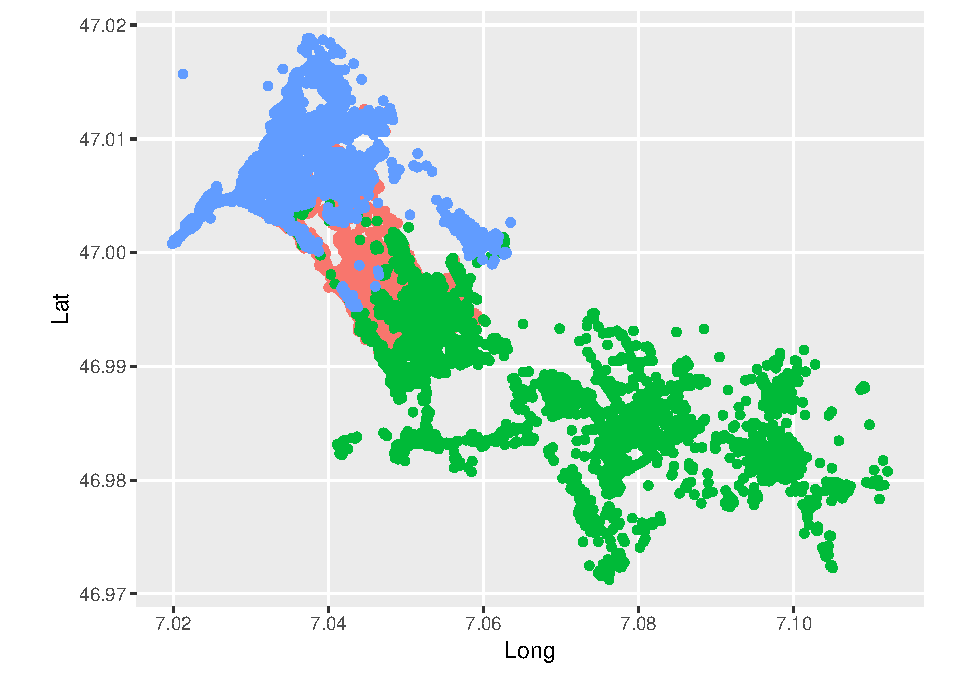
\includegraphics{patterns-and-trends_files/figure-latex/unnamed-chunk-11-1.pdf}

\subsection{Input: Handling spatial
data}\label{input-handling-spatial-data}

Until now, we've stored our location data within data frames as Lat/Long
columns. This works well for many tasks, but sometimes we need special
\emph{spatial} classes to handle our trajectories. We will get to know
such cases in our next tasks, but first we need to convert our
\texttt{data.frame} into a spatial object. Some of you might be familiar
with the \texttt{sp} package with the classes \texttt{SpatialPoints},
\texttt{SpatialPointsDataFrame} and so on. These packages are mostly
replaced by the fairly new package \texttt{sf}. This packages has some
huge advantages over \texttt{sp}:

\begin{itemize}
\tightlist
\item
  simple features are essentially data frames with minor extensions and
  thus are easily integratable in standard workflows
\item
  they are programmed to cleanly interface with the \texttt{tidyverse}
  methods (specifically \texttt{dplyr}'s \texttt{mutate} and
  \texttt{summarise})
\item
  comply with the common Open Geospatial Consortium (OGC) standards (ISO
  19125-1:2004) and interface with other important spatial tools such as
  GDAL, PostGIS, GeoJSON and so fourth
\item
  are being rapidly implemented in visualisation tools such as
  \texttt{ggplot2}, \texttt{plotly} and \texttt{tmap}
\end{itemize}

We will largely rely on \texttt{sf}when working with vector data in
\texttt{R}. In order to transform our \texttt{data.frame} into an sf
object, we need to use the function \texttt{st\_as\_sf()} while
specifying the columns storing the coordinates and the coordinate
reference system\footnote{At this point, we assume you know what a
  Coordinate Reference Systems is. Check out
  \href{https://earthdatascience.org/courses/earth-analytics/spatial-data-r/intro-to-coordinate-reference-systems/}{this
  link} if this is not the case.}.

\begin{Shaded}
\begin{Highlighting}[]
\KeywordTok{library}\NormalTok{(sf)}

\NormalTok{wildschwein_BE_sf <-}\StringTok{ }\KeywordTok{st_as_sf}\NormalTok{(wildschwein_BE, }\DataTypeTok{coords =} \KeywordTok{c}\NormalTok{(}\StringTok{"Long"}\NormalTok{, }\StringTok{"Lat"}\NormalTok{), }\DataTypeTok{crs =} \DecValTok{4326}\NormalTok{)}
\end{Highlighting}
\end{Shaded}

Notice how \texttt{st\_as\_sf} takes the EPSG code for the
\texttt{crs\ =} argument. This is so much easier and more elegant than
using \texttt{PROJ.4} or \texttt{WKT}. You can find a lot of useful
information on Coordinate Reference Systems (including EPSG Codes ,
etc.) under
\href{http://spatialreference.org/ref/epsg/2056/}{spatialreference.org}
or \url{http://epsg.io}.

Let's compare our original \texttt{data.frame} with this new \texttt{sf}
object:

\begin{Shaded}
\begin{Highlighting}[]
\NormalTok{wildschwein_BE}
\end{Highlighting}
\end{Shaded}

\begin{verbatim}
## # A tibble: 51,246 x 6
##    TierID TierName CollarID DatetimeUTC           Lat  Long
##    <chr>  <chr>       <dbl> <dttm>              <dbl> <dbl>
##  1 002A   Sabi        12275 2014-08-22 21:00:12  47.0  7.05
##  2 002A   Sabi        12275 2014-08-22 21:15:16  47.0  7.05
##  3 002A   Sabi        12275 2014-08-22 21:30:43  47.0  7.05
##  4 002A   Sabi        12275 2014-08-22 21:46:07  47.0  7.05
##  5 002A   Sabi        12275 2014-08-22 22:00:22  47.0  7.05
##  6 002A   Sabi        12275 2014-08-22 22:15:10  47.0  7.05
##  7 002A   Sabi        12275 2014-08-22 22:30:13  47.0  7.05
##  8 002A   Sabi        12275 2014-08-22 22:45:11  47.0  7.05
##  9 002A   Sabi        12275 2014-08-22 23:00:27  47.0  7.05
## 10 002A   Sabi        12275 2014-08-22 23:15:41  47.0  7.05
## # ... with 51,236 more rows
\end{verbatim}

\begin{Shaded}
\begin{Highlighting}[]
\NormalTok{wildschwein_BE_sf}
\end{Highlighting}
\end{Shaded}

\begin{verbatim}
## Simple feature collection with 51246 features and 4 fields
## geometry type:  POINT
## dimension:      XY
## bbox:           xmin: 7.019889 ymin: 46.97125 xmax: 7.112075 ymax: 47.01882
## epsg (SRID):    4326
## proj4string:    +proj=longlat +datum=WGS84 +no_defs
## # A tibble: 51,246 x 5
##    TierID TierName CollarID DatetimeUTC                    geometry
##    <chr>  <chr>       <dbl> <dttm>                      <POINT [°]>
##  1 002A   Sabi        12275 2014-08-22 21:00:12 (7.049618 46.99317)
##  2 002A   Sabi        12275 2014-08-22 21:15:16 (7.049509 46.99416)
##  3 002A   Sabi        12275 2014-08-22 21:30:43 (7.049406 46.99383)
##  4 002A   Sabi        12275 2014-08-22 21:46:07 (7.049217 46.99375)
##  5 002A   Sabi        12275 2014-08-22 22:00:22 (7.049359 46.99375)
##  6 002A   Sabi        12275 2014-08-22 22:15:10 (7.049363 46.99382)
##  7 002A   Sabi        12275 2014-08-22 22:30:13 (7.049326 46.99387)
##  8 002A   Sabi        12275 2014-08-22 22:45:11 (7.049237 46.99395)
##  9 002A   Sabi        12275 2014-08-22 23:00:27 (7.048383 46.99481)
## 10 002A   Sabi        12275 2014-08-22 23:15:41 (7.049396 46.99373)
## # ... with 51,236 more rows
\end{verbatim}

As you can see, \texttt{st\_as\_sf()} has added some metadata to our
dataframe (\texttt{geometry\ type}, \texttt{dimension}, \texttt{bbox},
\texttt{epsg} and \texttt{proj4string}) and replaced the columns
\texttt{Lat} and \texttt{Long} with a column named \texttt{geometry}.
Other than that, the new \texttt{sf} object is very similar to our
original dataframe. In fact, \texttt{sf} objects \emph{are} essentially
\texttt{dataframes}, just ask \texttt{R}:

\begin{Shaded}
\begin{Highlighting}[]
\KeywordTok{is.data.frame}\NormalTok{(wildschwein_BE_sf)}
\NormalTok{## [1] TRUE}
\end{Highlighting}
\end{Shaded}

All operations we know from handling \texttt{data.frames} can be used on
the \texttt{sf} object. Try some out!

\begin{Shaded}
\begin{Highlighting}[]
\CommentTok{# subset rows}
\NormalTok{wildschwein_BE_sf[}\DecValTok{1}\OperatorTok{:}\DecValTok{10}\NormalTok{,]}
\NormalTok{wildschwein_BE_sf[wildschwein_BE_sf}\OperatorTok{$}\NormalTok{TierName }\OperatorTok{==}\StringTok{ "Sabi"}\NormalTok{,]}

\CommentTok{# subset colums}
\NormalTok{wildschwein_BE_sf[,}\DecValTok{2}\OperatorTok{:}\DecValTok{3}\NormalTok{]}
\end{Highlighting}
\end{Shaded}

Instead of keeping the same data twice (once as a \texttt{data.frame},
and once as an \texttt{sf} object), we will overwrite the
\texttt{data.frame} and continue working with the \texttt{sf} object
from now on. This saves some memory space in \texttt{R} and avoids
confusion.

\begin{Shaded}
\begin{Highlighting}[]
\NormalTok{wildschwein_BE =}\StringTok{ }\KeywordTok{st_as_sf}\NormalTok{(wildschwein_BE, }\DataTypeTok{coords =} \KeywordTok{c}\NormalTok{(}\StringTok{"Long"}\NormalTok{, }\StringTok{"Lat"}\NormalTok{), }\DataTypeTok{crs =} \DecValTok{4326}\NormalTok{)}

\KeywordTok{rm}\NormalTok{(wildschwein_BE_sf) }\CommentTok{# we can remove this sf object, since it just eats up our memory}
\end{Highlighting}
\end{Shaded}

\subsection{Task 4: Project data from
WGS84}\label{task-4-project-data-from-wgs84}

So what can we do with our new \texttt{sf} object that we couldn't
before? One example is projecting the WGS84 (\texttt{Lat}/\texttt{Long})
coordinates into the new Swiss CRS \texttt{CH1903+\ LV95}\footnote{As
  we've mentioned in the first Input, you can look up the EPSG codes
  under
  \href{http://spatialreference.org/ref/epsg/2056/}{spatialreference.org}
  or \url{http://epsg.io}. For information specific to Switzerland,
  check the
  \href{https://www.swisstopo.admin.ch/en/knowledge-facts/surveying-geodesy/reference-systems.html}{swisstopo
  website}}. Do this by using the function \texttt{st\_transform}. By
the way, do you notice a pattern here? The package \texttt{sf} names
most functions for spatial operations with the prefix \texttt{st\_*},
just as in PostGIS.

Here's the resulting \texttt{sf} object from the operation:

\begin{verbatim}
## Simple feature collection with 51246 features and 4 fields
## geometry type:  POINT
## dimension:      XY
## bbox:           xmin: 2568153 ymin: 1202306 xmax: 2575154 ymax: 1207609
## epsg (SRID):    2056
## proj4string:    +proj=somerc +lat_0=46.95240555555556 +lon_0=7.439583333333333 +k_0=1 +x_0=2600000 +y_0=1200000 +ellps=bessel +towgs84=674.374,15.056,405.346,0,0,0,0 +units=m +no_defs
## # A tibble: 51,246 x 5
##    TierID TierName CollarID DatetimeUTC                  geometry
##    <chr>  <chr>       <dbl> <dttm>                    <POINT [m]>
##  1 002A   Sabi        12275 2014-08-22 21:00:12 (2570409 1204752)
##  2 002A   Sabi        12275 2014-08-22 21:15:16 (2570402 1204863)
##  3 002A   Sabi        12275 2014-08-22 21:30:43 (2570394 1204826)
##  4 002A   Sabi        12275 2014-08-22 21:46:07 (2570379 1204817)
##  5 002A   Sabi        12275 2014-08-22 22:00:22 (2570390 1204818)
##  6 002A   Sabi        12275 2014-08-22 22:15:10 (2570390 1204825)
##  7 002A   Sabi        12275 2014-08-22 22:30:13 (2570387 1204831)
##  8 002A   Sabi        12275 2014-08-22 22:45:11 (2570381 1204840)
##  9 002A   Sabi        12275 2014-08-22 23:00:27 (2570316 1204935)
## 10 002A   Sabi        12275 2014-08-22 23:15:41 (2570393 1204815)
## # ... with 51,236 more rows
\end{verbatim}

\subsection{Input: Calculate Convex
Hull}\label{input-calculate-convex-hull}

Transforming from one Coordinate Reference System to another was one
operation where we needed an object with a spatial nature. In this way,
we were able to use an off the shelf function to project the coordinates
from one CRS to another. In our next example, we again rely on a spatial
function: We want to calculate a
\href{https://en.wikipedia.org/wiki/Convex_hull}{convex hull} per Wild
boar. And guess what the function for calculating a convex hull is
called in \texttt{sf}? If you guessed \texttt{st\_convex\_hull()}, you
were right!

By default \texttt{st\_convex\_hull()} calculates the convex hull
\emph{per feature}, i.e. \emph{per point} in our dataset. This of course
makes little sense. In order to calculate the convex hull per animal, we
need to convert our point- to multipoint-features where each feature
contains all positions of one animal. This is achieved in two steps:

First: add a grouping variable to the \texttt{sf} object. Note the new
grouping variable in the metadata of the \texttt{sf} object. Other than
that, \texttt{group\_by} has no effect on our \texttt{sf} object.

\begin{Shaded}
\begin{Highlighting}[]
\NormalTok{wildschwein_BE_grouped <-}\StringTok{ }\KeywordTok{group_by}\NormalTok{(wildschwein_BE,TierID)}

\NormalTok{wildschwein_BE_grouped}
\NormalTok{## Simple feature collection with 51246 features and 4 fields}
\NormalTok{## geometry type:  POINT}
\NormalTok{## dimension:      XY}
\NormalTok{## bbox:           xmin: 2568153 ymin: 1202306 xmax: 2575154 ymax: 1207609}
\NormalTok{## epsg (SRID):    2056}
\NormalTok{## proj4string:    +proj=somerc +lat_0=46.95240555555556 +lon_0=7.439583333333333 +k_0=1 +x_0=2600000 +y_0=1200000 +ellps=bessel +towgs84=674.374,15.056,405.346,0,0,0,0 +units=m +no_defs}
\NormalTok{## # A tibble: 51,246 x 5}
\NormalTok{## # Groups:   TierID [3]}
\NormalTok{##    TierID TierName CollarID DatetimeUTC                  geometry}
\NormalTok{##    <chr>  <chr>       <dbl> <dttm>                    <POINT [m]>}
\NormalTok{##  1 002A   Sabi        12275 2014-08-22 21:00:12 (2570409 1204752)}
\NormalTok{##  2 002A   Sabi        12275 2014-08-22 21:15:16 (2570402 1204863)}
\NormalTok{##  3 002A   Sabi        12275 2014-08-22 21:30:43 (2570394 1204826)}
\NormalTok{##  4 002A   Sabi        12275 2014-08-22 21:46:07 (2570379 1204817)}
\NormalTok{##  5 002A   Sabi        12275 2014-08-22 22:00:22 (2570390 1204818)}
\NormalTok{##  6 002A   Sabi        12275 2014-08-22 22:15:10 (2570390 1204825)}
\NormalTok{##  7 002A   Sabi        12275 2014-08-22 22:30:13 (2570387 1204831)}
\NormalTok{##  8 002A   Sabi        12275 2014-08-22 22:45:11 (2570381 1204840)}
\NormalTok{##  9 002A   Sabi        12275 2014-08-22 23:00:27 (2570316 1204935)}
\NormalTok{## 10 002A   Sabi        12275 2014-08-22 23:15:41 (2570393 1204815)}
\NormalTok{## # ... with 51,236 more rows}
\end{Highlighting}
\end{Shaded}

Second: use \texttt{summarise()} to ``dissolve'' all points into a
mulipoint object.

\begin{Shaded}
\begin{Highlighting}[]
\NormalTok{wildschwein_BE_smry <-}\StringTok{ }\KeywordTok{summarise}\NormalTok{(wildschwein_BE_grouped)}

\NormalTok{wildschwein_BE_smry}
\NormalTok{## Simple feature collection with 3 features and 1 field}
\NormalTok{## geometry type:  MULTIPOINT}
\NormalTok{## dimension:      XY}
\NormalTok{## bbox:           xmin: 2568153 ymin: 1202306 xmax: 2575154 ymax: 1207609}
\NormalTok{## epsg (SRID):    2056}
\NormalTok{## proj4string:    +proj=somerc +lat_0=46.95240555555556 +lon_0=7.439583333333333 +k_0=1 +x_0=2600000 +y_0=1200000 +ellps=bessel +towgs84=674.374,15.056,405.346,0,0,0,0 +units=m +no_defs}
\NormalTok{## # A tibble: 3 x 2}
\NormalTok{##   TierID                                                           geometry}
\NormalTok{##   <chr>                                                    <MULTIPOINT [m]>}
\NormalTok{## 1 002A   (2568903 1206200, 2568925 1206207, 2568980 1206197, 2569024 12063~}
\NormalTok{## 2 016A   (2569231 1205823, 2569245 1205925, 2569247 1206027, 2569251 12058~}
\NormalTok{## 3 018A   (2568153 1205611, 2568155 1205613, 2568161 1205624, 2568162 12056~}
\end{Highlighting}
\end{Shaded}

Now we can run \texttt{st\_convex\_hull} on the new \texttt{sf} object.

\begin{Shaded}
\begin{Highlighting}[]
\NormalTok{mcp <-}\StringTok{ }\KeywordTok{st_convex_hull}\NormalTok{(wildschwein_BE_smry)}
\end{Highlighting}
\end{Shaded}

\subsection{Task 5: Ploting spatial
objects}\label{task-5-ploting-spatial-objects}

Using base plot to visualize \texttt{sf} objects is easy enough, just
try the following code.

\begin{Shaded}
\begin{Highlighting}[]
\KeywordTok{plot}\NormalTok{(mcp)}
\end{Highlighting}
\end{Shaded}

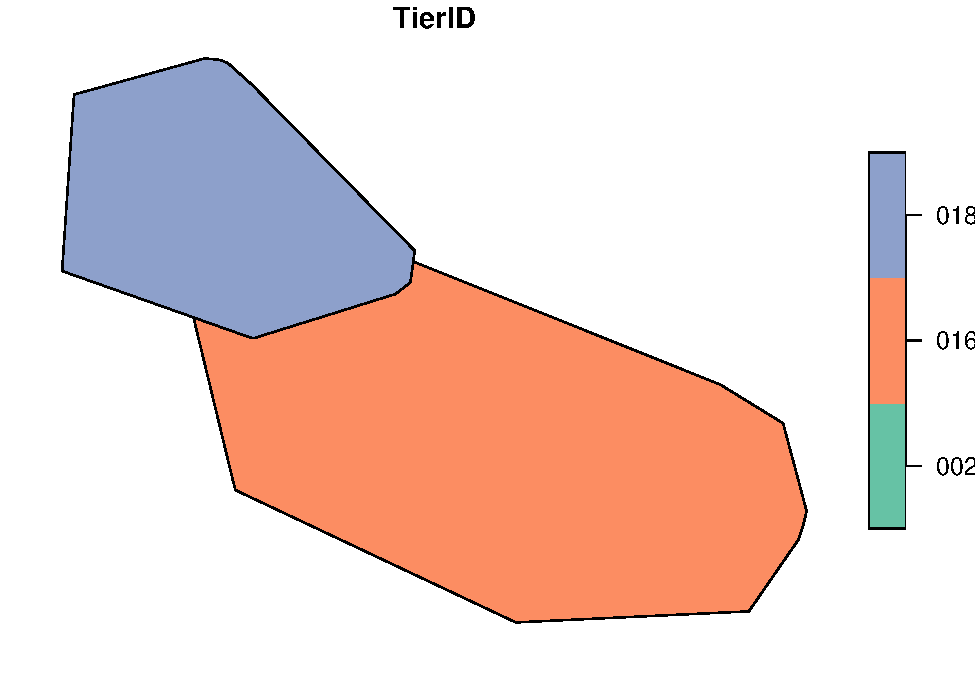
\includegraphics{patterns-and-trends_files/figure-latex/unnamed-chunk-30-1.pdf}

But since we use \texttt{ggplot} extensively, try and plot the object
\texttt{mcp} with \texttt{ggplot}. Hint: Use the layer
\texttt{geom\_sf()} to add an \texttt{sf} object.

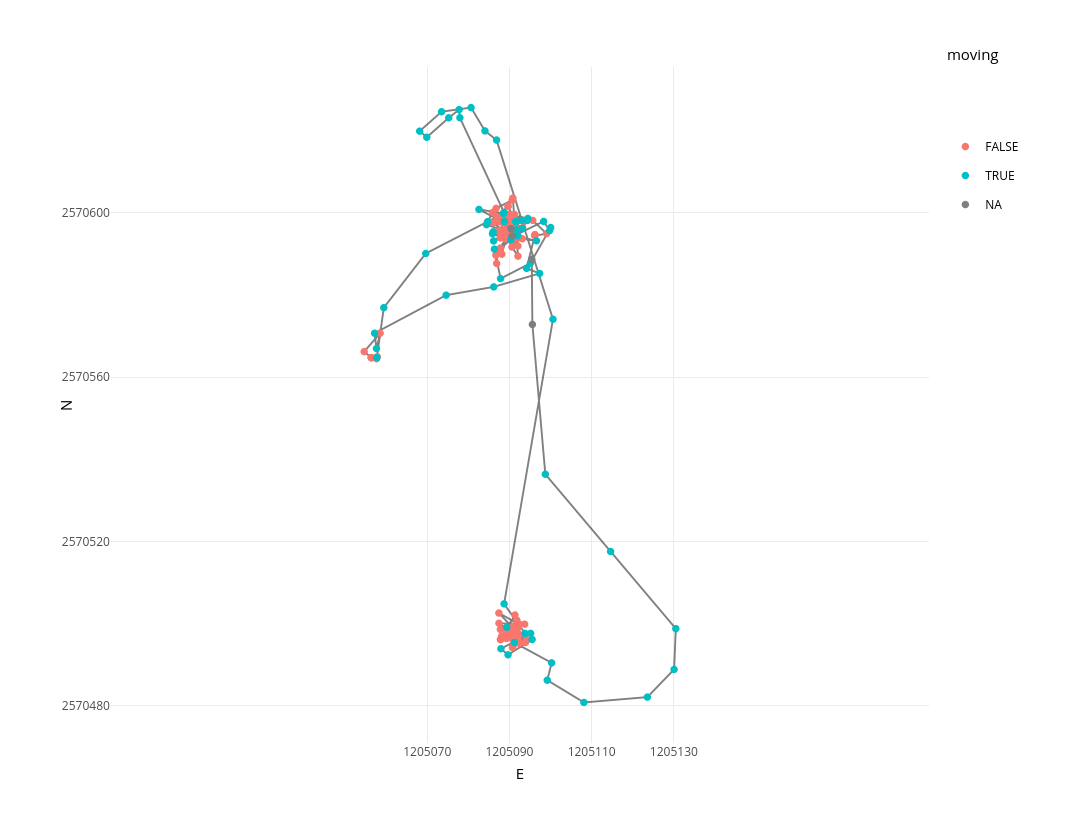
\includegraphics{patterns-and-trends_files/figure-latex/unnamed-chunk-31-1.pdf}

Note: \texttt{ggplot} refuses to use our specified CRS, so we need to
force this by specifying \texttt{datum\ =} in \texttt{coord\_sf()}. Try
it out.

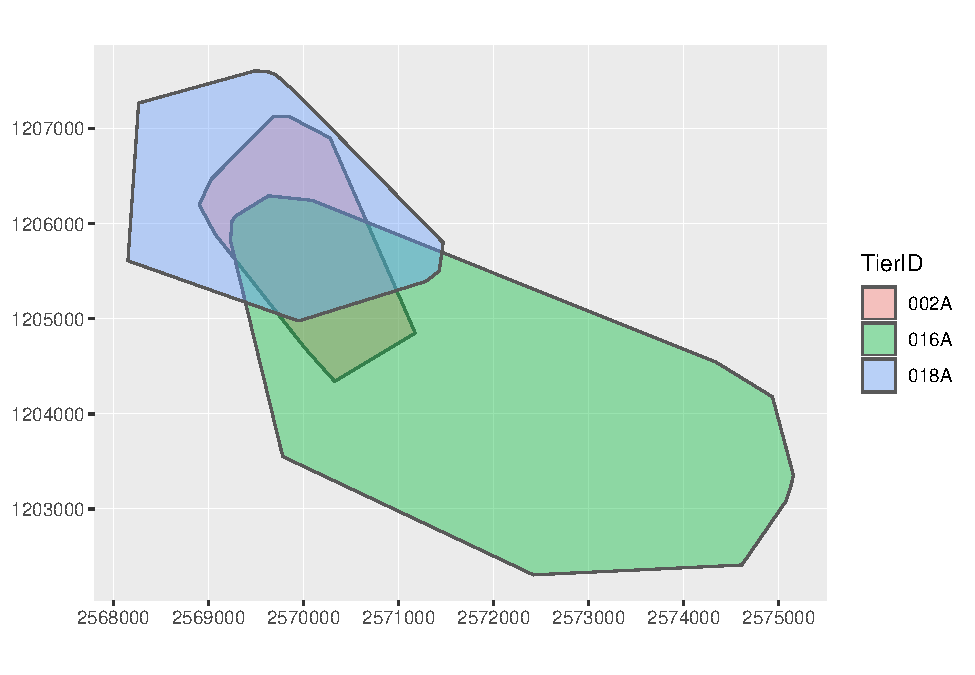
\includegraphics{patterns-and-trends_files/figure-latex/unnamed-chunk-32-1.pdf}

\subsection{Input: Importing raster
data}\label{input-importing-raster-data}

In the next task, we would like to add a background map to our
\texttt{mcp} object. To do this, we have to the raster data into
\texttt{R} first. For this, we use the package \texttt{raster} with the
function \texttt{brick}.

\begin{Shaded}
\begin{Highlighting}[]

\KeywordTok{library}\NormalTok{(raster)}

\NormalTok{pk100_BE <-}\StringTok{ }\KeywordTok{brick}\NormalTok{(}\StringTok{"00_Rawdata/pk100_BE_2056.tif"}\NormalTok{)}

\NormalTok{pk100_BE}
\NormalTok{## class       : RasterBrick }
\NormalTok{## dimensions  : 1821, 2321, 4226541, 4  (nrow, ncol, ncell, nlayers)}
\NormalTok{## resolution  : 5, 5  (x, y)}
\NormalTok{## extent      : 2567000, 2578605, 1199996, 1209101  (xmin, xmax, ymin, ymax)}
\NormalTok{## coord. ref. : +proj=somerc +lat_0=46.95240555555556 +lon_0=7.439583333333333 +k_0=1 +x_0=2600000 +y_0=1200000 +ellps=bessel +towgs84=674.374,15.056,405.346,0,0,0,0 +units=m +no_defs }
\NormalTok{## data source : /home/staff/rata/unix/Master/PatternsAndTrends/2019_FS/Unterrichtsunterlagen/00_Rawdata/pk100_BE_2056.tif }
\NormalTok{## names       : pk100_BE_2056.1, pk100_BE_2056.2, pk100_BE_2056.3, pk100_BE_2056.4 }
\NormalTok{## min values  :               0,               0,               0,               0 }
\NormalTok{## max values  :             255,             255,             255,             255}
\end{Highlighting}
\end{Shaded}

\texttt{pk100\_BE\_2056.tif} is a three layered geotiff File. The above
console output shows some metadata including the resolution, extent and
the names of our layers (\texttt{pk100\_BE\_2056.1},
\texttt{pk100\_BE\_2056.2}etc). For some reason, \texttt{RasterBrick}
imported a fourth layer (\texttt{pk100\_BE\_2056.4}). \texttt{plot()}
shows that the fourth layer is empty. We will remove this layer using
\texttt{subset()}.

\begin{Shaded}
\begin{Highlighting}[]

\KeywordTok{plot}\NormalTok{(pk100_BE)}
\end{Highlighting}
\end{Shaded}

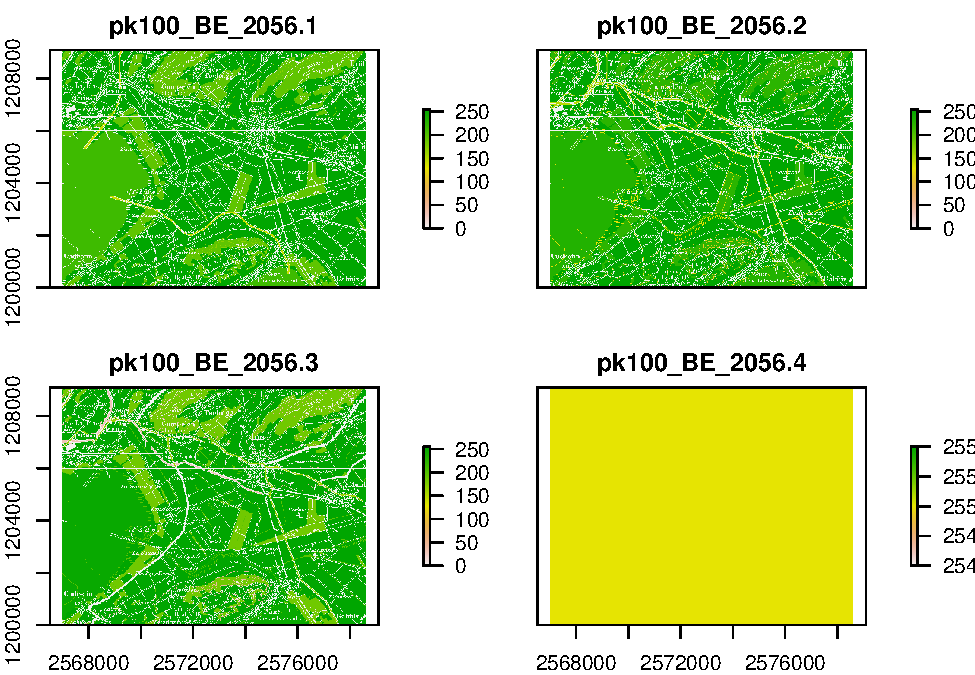
\includegraphics{patterns-and-trends_files/figure-latex/unnamed-chunk-36-1.pdf}

\begin{Shaded}
\begin{Highlighting}[]

\NormalTok{pk100_BE <-}\StringTok{ }\KeywordTok{subset}\NormalTok{(pk100_BE,}\DecValTok{1}\OperatorTok{:}\DecValTok{3}\NormalTok{)}

\KeywordTok{plot}\NormalTok{(pk100_BE)}
\end{Highlighting}
\end{Shaded}

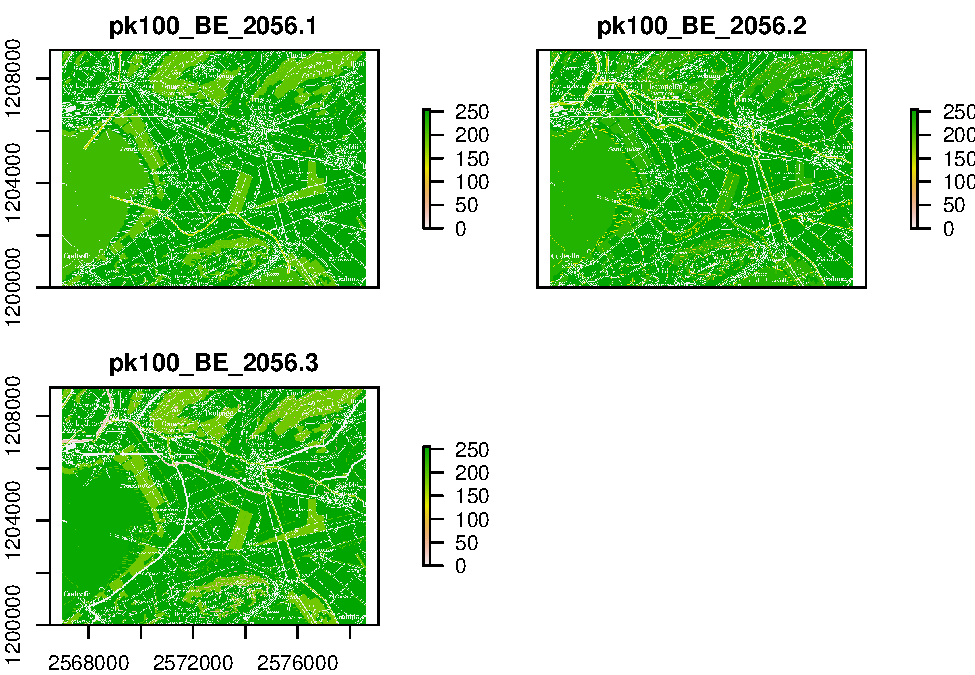
\includegraphics{patterns-and-trends_files/figure-latex/unnamed-chunk-36-2.pdf}

\subsection{Task 6: Adding a background
map}\label{task-6-adding-a-background-map}

There are multiple ways to add a background map in \texttt{ggplot}, many
require additional packages. This is a good opportunity to get to know a
completely different package for creating maps: \texttt{tmap}
(``thematic map''). This package was developed with a syntax very
similar to \texttt{ggplot2}, which makes it easy to learn.

\begin{Shaded}
\begin{Highlighting}[]
\KeywordTok{library}\NormalTok{(tmap)}


\KeywordTok{tm_shape}\NormalTok{(pk100_BE) }\OperatorTok{+}\StringTok{ }
\StringTok{  }\KeywordTok{tm_rgb}\NormalTok{() }
\end{Highlighting}
\end{Shaded}

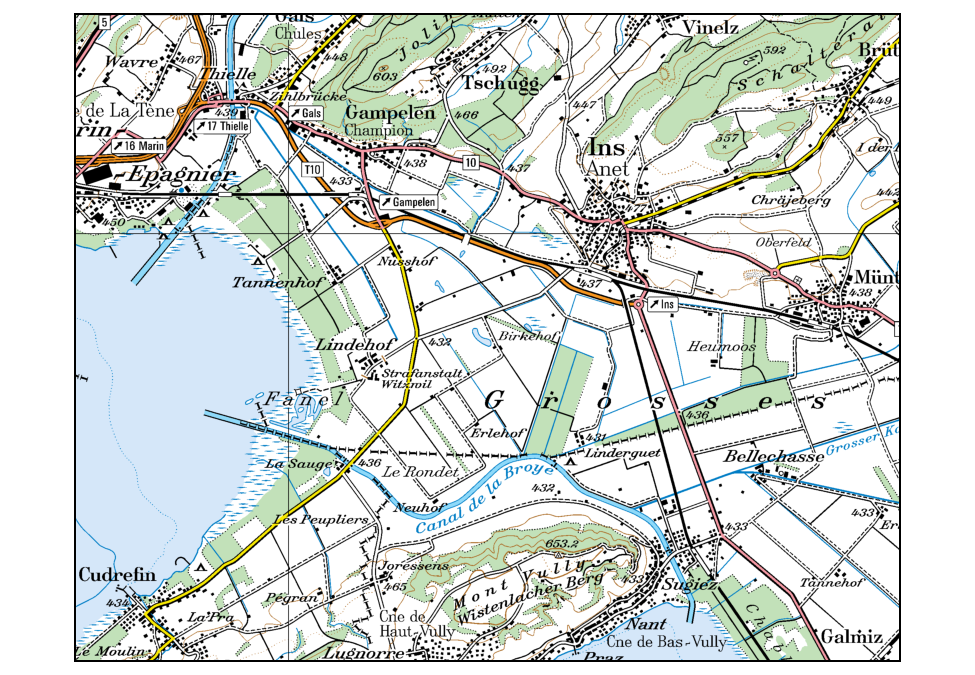
\includegraphics{patterns-and-trends_files/figure-latex/unnamed-chunk-39-1.pdf}

As you can see, plotting layers in \texttt{tmap} is combined with the
\texttt{+} sign, just as in \texttt{ggplot2}. In \texttt{tmap} however,
each layer consists of two objects: a \texttt{tm\_shape()} in which the
data is called, and a \texttt{tm\_*} object in which we define how the
data is visualized (\texttt{tm\_rgb()} states that it is plotted as an
RGB Raster Layer). Add the object \texttt{mcp} to the plot in this
manner. Read
\href{https://cran.r-project.org/web/packages/tmap/vignettes/tmap-getstarted.html}{the
vignette} if you are having trouble.

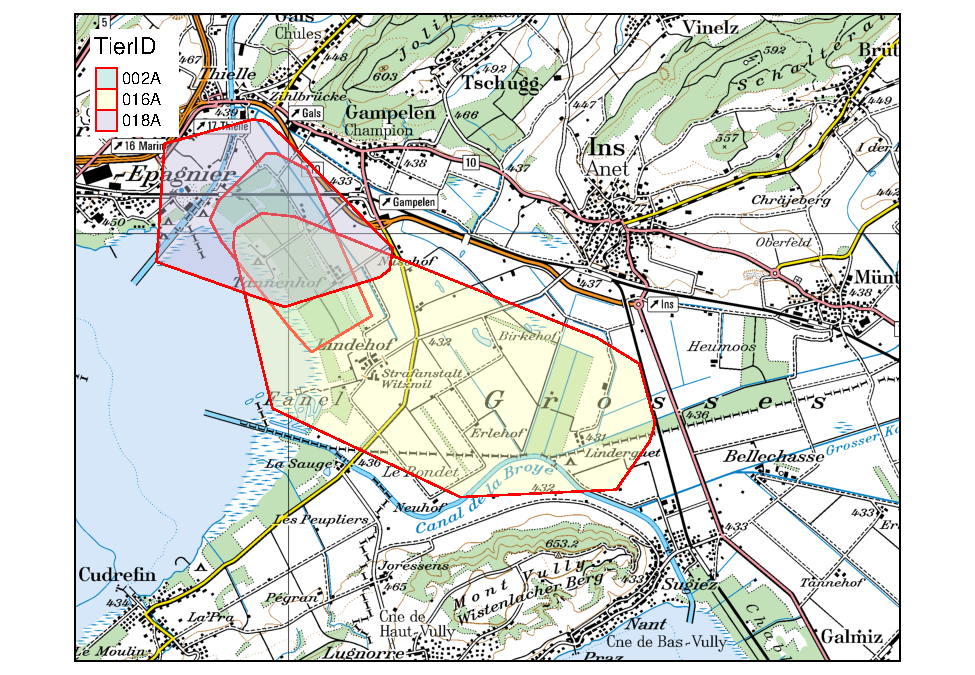
\includegraphics{patterns-and-trends_files/figure-latex/unnamed-chunk-40-1.pdf}

\subsection{Task 7: Create an interactive
map}\label{task-7-create-an-interactive-map}

Rerun the \texttt{tmap()...} command from the previous task, but switch
the plotting mode to ``view''" (\texttt{tmap\_mode("view")}) beforehand.

\chapter{Exercise 2}\label{exercise-2}

\section{Learning Outcomes}\label{learning-outcomes}

\begin{itemize}
\tightlist
\item
  You understand the dplyr functions \texttt{mutate}, \texttt{summarise}
  and \texttt{group\_by} and can apply them to \texttt{sf} objects
\item
  You can derive movement parameters (\texttt{timelag},
  \texttt{steplength}, \texttt{speed}) from trajectory data.
\item
  You can re-sample your trajectory data for cross scale movement
  analysis.
\end{itemize}

\section{Prerequisites}\label{prerequisites-1}

Readings Skills from ``R for Data Science'' (Wickham and Grolemund
\protect\hyperlink{ref-wickham2017}{2017}):

\begin{itemize}
\tightlist
\item
  RS2.1 Chap3 Data Transformation with \texttt{dplyr} (31p, 43-76)
\item
  RS2.2 Chap10 Relational data with \texttt{dplyr} (21p, 171-193)
\item
  RS2.3 Chap14 Pipes with \texttt{magrittr} (6p, 261-268)
\end{itemize}

Readings Theory

\begin{itemize}
\tightlist
\item
  R2.1 Laube and Purves (\protect\hyperlink{ref-laube2011}{2011}): How
  fast is a cow? cross - scale analysis of movement data.
\end{itemize}

\section{Preperation}\label{preperation-1}

Install the package \texttt{zoo} to get access to the rolling window
functions for last exercise.

\begin{Shaded}
\begin{Highlighting}[]
\KeywordTok{install.packages}\NormalTok{(}\StringTok{"zoo"}\NormalTok{)}
\end{Highlighting}
\end{Shaded}

Import the wild boar data and convert it to an \texttt{sf} object with
CH1903+ LV95 Coordinates. Either run your own script from last week or
the following lines to bring the data to the form we need it for today
exercise.

\begin{Shaded}
\begin{Highlighting}[]
\KeywordTok{library}\NormalTok{(tidyverse)}
\KeywordTok{library}\NormalTok{(sf)}
\KeywordTok{library}\NormalTok{(lubridate)}

\NormalTok{wildschwein_BE <-}\StringTok{ }\KeywordTok{read_delim}\NormalTok{(}\StringTok{"00_Rawdata/wildschwein_BE.csv"}\NormalTok{,}\StringTok{","}\NormalTok{)}

\NormalTok{wildschwein_BE =}\StringTok{ }\KeywordTok{st_as_sf}\NormalTok{(wildschwein_BE, }\DataTypeTok{coords =} \KeywordTok{c}\NormalTok{(}\StringTok{"Long"}\NormalTok{, }\StringTok{"Lat"}\NormalTok{), }\DataTypeTok{crs =} \DecValTok{4326}\NormalTok{)}

\NormalTok{wildschwein_BE <-}\StringTok{ }\KeywordTok{st_transform}\NormalTok{(wildschwein_BE, }\DecValTok{2056}\NormalTok{)}
\end{Highlighting}
\end{Shaded}

\section{Demo Tidyverse}\label{demo-tidyverse}

Depending on your knowledge of \texttt{R}, getting an overview of the
data we imported last week might have been quite a challenge.
Surprisingly enough, importing, cleaning and exploring your data can be
the most challenging, time consuming part of a project. RStudio and the
tidyverse offer many helpful tools to make this part easier (and more
fun). You have read chapters on \texttt{dplyr} and \texttt{magrittr} as
a preparation for this Exercise. Before we start with the Exercise
however, this demo illustrates a simple approach offered by tidyverse
which is applicable to sf-objects.

Assume we want to calculate the timelag in between subsequent positions.
To achieve this we can use the function \texttt{difftime()} combined
with \texttt{lead()} from \texttt{dplyr}. Let's look at these functions
one by one.

\subsection{\texorpdfstring{\texttt{difftime}}{difftime}}\label{difftime}

\texttt{difftime} takes two \texttt{POSIXct} values.

\begin{Shaded}
\begin{Highlighting}[]
\NormalTok{now <-}\StringTok{ }\KeywordTok{Sys.time}\NormalTok{()}

\NormalTok{later <-}\StringTok{ }\NormalTok{now }\OperatorTok{+}\StringTok{ }\DecValTok{10000}

\NormalTok{time_difference <-}\StringTok{ }\KeywordTok{difftime}\NormalTok{(later,now)}
\end{Highlighting}
\end{Shaded}

You can also specify the unit of the output.

\begin{Shaded}
\begin{Highlighting}[]
\NormalTok{time_difference <-}\StringTok{ }\KeywordTok{difftime}\NormalTok{(later,now,}\DataTypeTok{units =} \StringTok{"mins"}\NormalTok{)}
\end{Highlighting}
\end{Shaded}

\texttt{difftime} returns an object of the Class \texttt{difftime}.
However in our case, numeric values would be more handy than the Class
\texttt{difftime}. So we'll wrap the command in \texttt{as.numeric()}:

\begin{Shaded}
\begin{Highlighting}[]
\KeywordTok{str}\NormalTok{(time_difference)}
\NormalTok{## Class 'difftime'  atomic [1:1] 167}
\NormalTok{##   ..- attr(*, "units")= chr "mins"}
\end{Highlighting}
\end{Shaded}

\begin{Shaded}
\begin{Highlighting}[]
\NormalTok{time_difference <-}\StringTok{ }\KeywordTok{as.numeric}\NormalTok{(}\KeywordTok{difftime}\NormalTok{(later,now,}\DataTypeTok{units =} \StringTok{"mins"}\NormalTok{))}

\KeywordTok{str}\NormalTok{(time_difference)}
\NormalTok{##  num 167}
\end{Highlighting}
\end{Shaded}

\subsection{\texorpdfstring{\texttt{lead()} /
\texttt{lag()}}{lead() / lag()}}\label{lead-lag}

\texttt{lead()} and \texttt{lag()} return a vector of the same length as
the input, just offset by a specific number of values (default is 1).
Consider the following sequence:

\begin{Shaded}
\begin{Highlighting}[]
\NormalTok{numbers <-}\StringTok{ }\DecValTok{1}\OperatorTok{:}\DecValTok{10}

\NormalTok{numbers}
\NormalTok{##  [1]  1  2  3  4  5  6  7  8  9 10}
\end{Highlighting}
\end{Shaded}

We can now run \texttt{lead()} and \texttt{lag()} on this sequence to
illustrate the output. \texttt{n\ =} specifies the offset,
\texttt{default\ =} specifies the default value used to ``fill'' the
emerging ``empty spaces'' of the vector.

\begin{Shaded}
\begin{Highlighting}[]
\KeywordTok{lead}\NormalTok{(numbers)}
\NormalTok{##  [1]  2  3  4  5  6  7  8  9 10 NA}

\KeywordTok{lead}\NormalTok{(numbers,}\DataTypeTok{n =} \DecValTok{2}\NormalTok{)}
\NormalTok{##  [1]  3  4  5  6  7  8  9 10 NA NA}

\KeywordTok{lag}\NormalTok{(numbers)}
\NormalTok{##  [1] NA  1  2  3  4  5  6  7  8  9}

\KeywordTok{lag}\NormalTok{(numbers,}\DataTypeTok{n =} \DecValTok{5}\NormalTok{)}
\NormalTok{##  [1] NA NA NA NA NA  1  2  3  4  5}

\KeywordTok{lag}\NormalTok{(numbers,}\DataTypeTok{n =} \DecValTok{5}\NormalTok{, }\DataTypeTok{default =} \DecValTok{0}\NormalTok{)}
\NormalTok{##  [1] 0 0 0 0 0 1 2 3 4 5}
\end{Highlighting}
\end{Shaded}

This helps us performing operations on subsequent values in a vector (or
rows in a table). You can think of this a little bit like a moving
temporal window that moves along the trajectory, or down the rows of a
table respectively.

\subsection{\texorpdfstring{\texttt{mutate()}}{mutate()}}\label{mutate}

Using the above functions (\texttt{difftime()} and \texttt{lead()}), we
can calculate the time lag, that is, the time difference between
subsequent positions:

\begin{Shaded}
\begin{Highlighting}[]

\NormalTok{wildschwein_BE}\OperatorTok{$}\NormalTok{timelag  <-}\StringTok{ }\KeywordTok{as.numeric}\NormalTok{(}\KeywordTok{difftime}\NormalTok{(}\KeywordTok{lead}\NormalTok{(wildschwein_BE}\OperatorTok{$}\NormalTok{DatetimeUTC),wildschwein_BE}\OperatorTok{$}\NormalTok{DatetimeUTC,}\DataTypeTok{units =} \StringTok{"secs"}\NormalTok{))}
\end{Highlighting}
\end{Shaded}

We mention \texttt{wildschwein\_BE} three times in this function, which
is complicated. Instead, we can use \texttt{mutate()} to simplify the
syntax:

\begin{Shaded}
\begin{Highlighting}[]
\NormalTok{wildschwein_BE <-}\StringTok{ }\KeywordTok{mutate}\NormalTok{(wildschwein_BE,}\DataTypeTok{timelag =} \KeywordTok{as.numeric}\NormalTok{(}\KeywordTok{difftime}\NormalTok{(}\KeywordTok{lead}\NormalTok{(DatetimeUTC),DatetimeUTC,}\DataTypeTok{units =} \StringTok{"secs"}\NormalTok{)))}
\end{Highlighting}
\end{Shaded}

\subsection{\texorpdfstring{\texttt{group\_by()}}{group\_by()}}\label{group_by}

Now let's have a look at the vector created before:

\begin{Shaded}
\begin{Highlighting}[]
\KeywordTok{summary}\NormalTok{(wildschwein_BE}\OperatorTok{$}\NormalTok{timelag)}
\NormalTok{##      Min.   1st Qu.    Median      Mean   3rd Qu.      Max.      NA's }
\NormalTok{## -22648470       896       903       571       916     60367         1}
\end{Highlighting}
\end{Shaded}

These values don't make much sense: some are negative (which should not
be the case) and some are very high (which would indicate large data
gaps and should not be the case either). The reason for this result is
that we did not consider that \texttt{timelag} should just be calculated
between subsequent rows \emph{of the same individual}. We can implement
this by using \texttt{group\_by()} (just as if calculating the convex
hull last week).

\begin{Shaded}
\begin{Highlighting}[]
\NormalTok{wildschwein_BE <-}\StringTok{ }\KeywordTok{group_by}\NormalTok{(wildschwein_BE,TierID)}
\end{Highlighting}
\end{Shaded}

After adding this grouping variable, calculating the timelag
automatically accounts for the individual trajectories.

\begin{Shaded}
\begin{Highlighting}[]
\NormalTok{wildschwein_BE <-}\StringTok{ }\KeywordTok{mutate}\NormalTok{(wildschwein_BE,}\DataTypeTok{timelag =} \KeywordTok{as.numeric}\NormalTok{(}\KeywordTok{difftime}\NormalTok{(}\KeywordTok{lead}\NormalTok{(DatetimeUTC),DatetimeUTC,}\DataTypeTok{units =} \StringTok{"secs"}\NormalTok{)))}

\KeywordTok{summary}\NormalTok{(wildschwein_BE}\OperatorTok{$}\NormalTok{timelag)}
\NormalTok{##    Min. 1st Qu.  Median    Mean 3rd Qu.    Max.    NA's }
\NormalTok{##      12     896     903    1408     916   60367       3}
\end{Highlighting}
\end{Shaded}

\subsection{\texorpdfstring{\texttt{summarise()}}{summarise()}}\label{summarise}

\texttt{summary()} returned the metrics over all individuals. If we want
to summarise our data and get metrics \emph{per animal}, we can use the
\texttt{dplyr} function \texttt{summarise()}. In contrast to
\texttt{mutate()}, which just adds a new column to the dataset,
\texttt{summarise()} ``collapses'' the data to one row per individual
(specified by \texttt{group\_by}).

\begin{Shaded}
\begin{Highlighting}[]
\KeywordTok{summarise}\NormalTok{(wildschwein_BE, }\DataTypeTok{mean =} \KeywordTok{mean}\NormalTok{(timelag, }\DataTypeTok{na.rm =}\NormalTok{ T))}
\end{Highlighting}
\end{Shaded}

The above operation works fine on normal \texttt{data.frames}, but since
\texttt{wildschwein\_BE} is also an \texttt{sf} object,
\texttt{summarise} actually merges all the points to a multipoint
geometry, which takes a long time to calculate. In order to prevent
this, we can set the objects geometry to \texttt{NULL}, which removes
the spatial attribute.

\begin{Shaded}
\begin{Highlighting}[]

\KeywordTok{summarise}\NormalTok{(}\KeywordTok{st_set_geometry}\NormalTok{(wildschwein_BE,}\OtherTok{NULL}\NormalTok{), }\DataTypeTok{mean_timelag =} \KeywordTok{mean}\NormalTok{(timelag, }\DataTypeTok{na.rm =}\NormalTok{ T))}
\NormalTok{## # A tibble: 3 x 2}
\NormalTok{##   TierID mean_timelag}
\NormalTok{##   <chr>         <dbl>}
\NormalTok{## 1 002A          1286.}
\NormalTok{## 2 016A          1412.}
\NormalTok{## 3 018A          1599.}
\end{Highlighting}
\end{Shaded}

\subsection{Piping}\label{piping}

The code above hard to read, since it has so many nested functions which
need to be read from the inside out. In order to make code readable in a
more human-friendly way, we can use the piping command
\texttt{\%\textgreater{}\%} from \texttt{magrittr}, which is included in
\texttt{dplyr} and the \texttt{tidyverse}. The above code then looks
like this:

\begin{Shaded}
\begin{Highlighting}[]

\NormalTok{wildschwein_BE }\OperatorTok\StringTok{                     }\CommentTok{# Take wildschwein_BE...}
\StringTok{  }\KeywordTok{st_set_geometry}\NormalTok{(}\OtherTok{NULL}\NormalTok{) }\OperatorTok\StringTok{            }\CommentTok{# ...remove the geometry column...}
\StringTok{  }\KeywordTok{group_by}\NormalTok{(TierID) }\OperatorTok\StringTok{                 }\CommentTok{# ...group it by TierID}
\StringTok{  }\KeywordTok{summarise}\NormalTok{(                           }\CommentTok{# Summarise the data...}
    \DataTypeTok{mean_timelag =} \KeywordTok{mean}\NormalTok{(timelag,}\DataTypeTok{na.rm =}\NormalTok{ T) }\CommentTok{# ...by calculating the mean timelag}
\NormalTok{  )}
\NormalTok{## # A tibble: 3 x 2}
\NormalTok{##   TierID mean_timelag}
\NormalTok{##   <chr>         <dbl>}
\NormalTok{## 1 002A          1286.}
\NormalTok{## 2 016A          1412.}
\NormalTok{## 3 018A          1599.}
\end{Highlighting}
\end{Shaded}

\subsection{Bring it all together\ldots{}}\label{bring-it-all-together}

Here is the same approach with a different, smaller dataset:

\begin{Shaded}
\begin{Highlighting}[]
\NormalTok{pigs =}\StringTok{ }\KeywordTok{data.frame}\NormalTok{(}
  \DataTypeTok{TierID=}\KeywordTok{c}\NormalTok{(}\DecValTok{8001}\NormalTok{,}\DecValTok{8003}\NormalTok{,}\DecValTok{8004}\NormalTok{,}\DecValTok{8005}\NormalTok{,}\DecValTok{8800}\NormalTok{,}\DecValTok{8820}\NormalTok{,}\DecValTok{3000}\NormalTok{,}\DecValTok{3001}\NormalTok{,}\DecValTok{3002}\NormalTok{,}\DecValTok{3003}\NormalTok{,}\DecValTok{8330}\NormalTok{,}\DecValTok{7222}\NormalTok{),}
  \DataTypeTok{sex=}\KeywordTok{c}\NormalTok{(}\StringTok{"M"}\NormalTok{,}\StringTok{"M"}\NormalTok{,}\StringTok{"M"}\NormalTok{,}\StringTok{"F"}\NormalTok{,}\StringTok{"M"}\NormalTok{,}\StringTok{"M"}\NormalTok{,}\StringTok{"F"}\NormalTok{,}\StringTok{"F"}\NormalTok{,}\StringTok{"M"}\NormalTok{,}\StringTok{"F"}\NormalTok{,}\StringTok{"M"}\NormalTok{,}\StringTok{"F"}\NormalTok{),}
  \DataTypeTok{age=}\KeywordTok{c}\NormalTok{(}\StringTok{"A"}\NormalTok{,}\StringTok{"A"}\NormalTok{,}\StringTok{"J"}\NormalTok{,}\StringTok{"A"}\NormalTok{,}\StringTok{"J"}\NormalTok{,}\StringTok{"J"}\NormalTok{,}\StringTok{"J"}\NormalTok{,}\StringTok{"A"}\NormalTok{,}\StringTok{"J"}\NormalTok{,}\StringTok{"J"}\NormalTok{,}\StringTok{"A"}\NormalTok{,}\StringTok{"A"}\NormalTok{),}
  \DataTypeTok{weight=}\KeywordTok{c}\NormalTok{(}\FloatTok{50.755}\NormalTok{,}\FloatTok{43.409}\NormalTok{,}\FloatTok{12.000}\NormalTok{,}\FloatTok{16.787}\NormalTok{,}\FloatTok{20.987}\NormalTok{,}\FloatTok{25.765}\NormalTok{,}\FloatTok{22.0122}\NormalTok{,}\FloatTok{21.343}\NormalTok{,}\FloatTok{12.532}\NormalTok{,}\FloatTok{54.32}\NormalTok{,}\FloatTok{11.027}\NormalTok{,}\FloatTok{88.08}\NormalTok{)}
\NormalTok{)}

\NormalTok{pigs}
\NormalTok{##    TierID sex age  weight}
\NormalTok{## 1    8001   M   A 50.7550}
\NormalTok{## 2    8003   M   A 43.4090}
\NormalTok{## 3    8004   M   J 12.0000}
\NormalTok{## 4    8005   F   A 16.7870}
\NormalTok{## 5    8800   M   J 20.9870}
\NormalTok{## 6    8820   M   J 25.7650}
\NormalTok{## 7    3000   F   J 22.0122}
\NormalTok{## 8    3001   F   A 21.3430}
\NormalTok{## 9    3002   M   J 12.5320}
\NormalTok{## 10   3003   F   J 54.3200}
\NormalTok{## 11   8330   M   A 11.0270}
\NormalTok{## 12   7222   F   A 88.0800}

\NormalTok{pigs }\OperatorTok
\StringTok{    }\KeywordTok{summarise}\NormalTok{(         }
    \DataTypeTok{mean_weight =} \KeywordTok{mean}\NormalTok{(weight)}
\NormalTok{  )}
\NormalTok{##   mean_weight}
\NormalTok{## 1    31.58477}

\NormalTok{pigs }\OperatorTok
\StringTok{  }\KeywordTok{group_by}\NormalTok{(sex) }\OperatorTok
\StringTok{  }\KeywordTok{summarise}\NormalTok{(         }
    \DataTypeTok{mean_weight =} \KeywordTok{mean}\NormalTok{(weight)}
\NormalTok{  )}
\NormalTok{## # A tibble: 2 x 2}
\NormalTok{##   sex   mean_weight}
\NormalTok{##   <fct>       <dbl>}
\NormalTok{## 1 F            40.5}
\NormalTok{## 2 M            25.2}

\NormalTok{pigs }\OperatorTok
\StringTok{  }\KeywordTok{group_by}\NormalTok{(sex,age) }\OperatorTok
\StringTok{  }\KeywordTok{summarise}\NormalTok{(         }
    \DataTypeTok{mean_weight =} \KeywordTok{mean}\NormalTok{(weight)}
\NormalTok{  )}
\NormalTok{## # A tibble: 4 x 3}
\NormalTok{## # Groups:   sex [?]}
\NormalTok{##   sex   age   mean_weight}
\NormalTok{##   <fct> <fct>       <dbl>}
\NormalTok{## 1 F     A            42.1}
\NormalTok{## 2 F     J            38.2}
\NormalTok{## 3 M     A            35.1}
\NormalTok{## 4 M     J            17.8}
\end{Highlighting}
\end{Shaded}

\section{Tasks and Inputs}\label{tasks-and-inputs-1}

\subsection{Task 1: Getting an
overview}\label{task-1-getting-an-overview}

Calculate the time difference between subsequent rows as described in
the demo (column \texttt{timelag}) First, inspect your data in more
detail. Try to answer the following questions:

\begin{itemize}
\tightlist
\item
  How many individuals were tracked?
\item
  How long were the individual tracked? Are there gaps?
\item
  Were all individuals tracked concurrently or sequentially?
\item
  What is the temporal sampling interval between the locations?
\end{itemize}

Here are some exemplary visualisation you could produce to answer these
questions. Can you now answer the above questions?
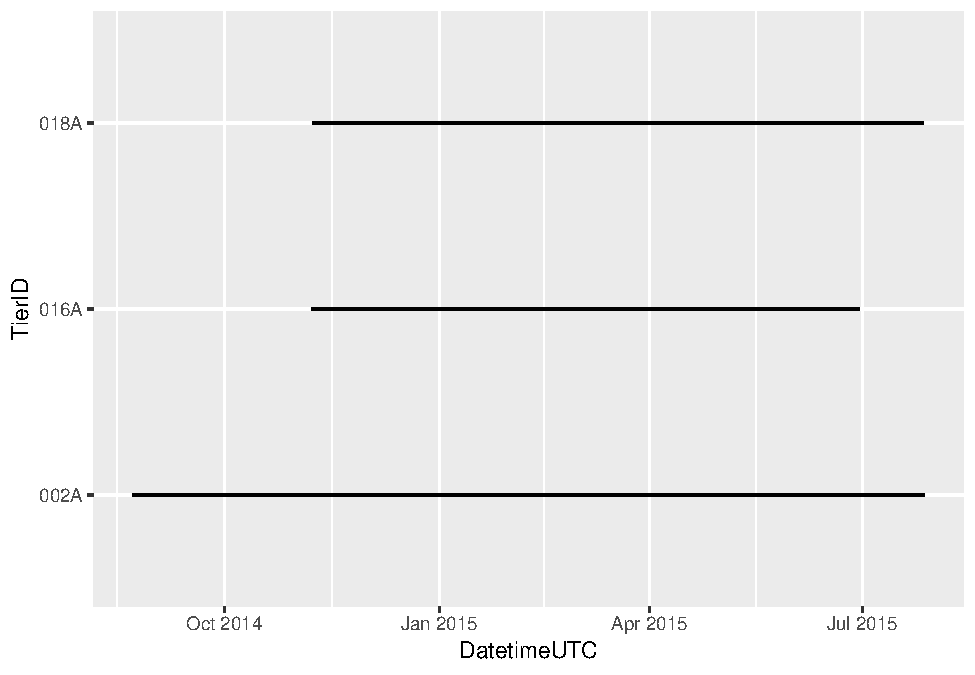
\includegraphics{patterns-and-trends_files/figure-latex/unnamed-chunk-69-1.pdf}
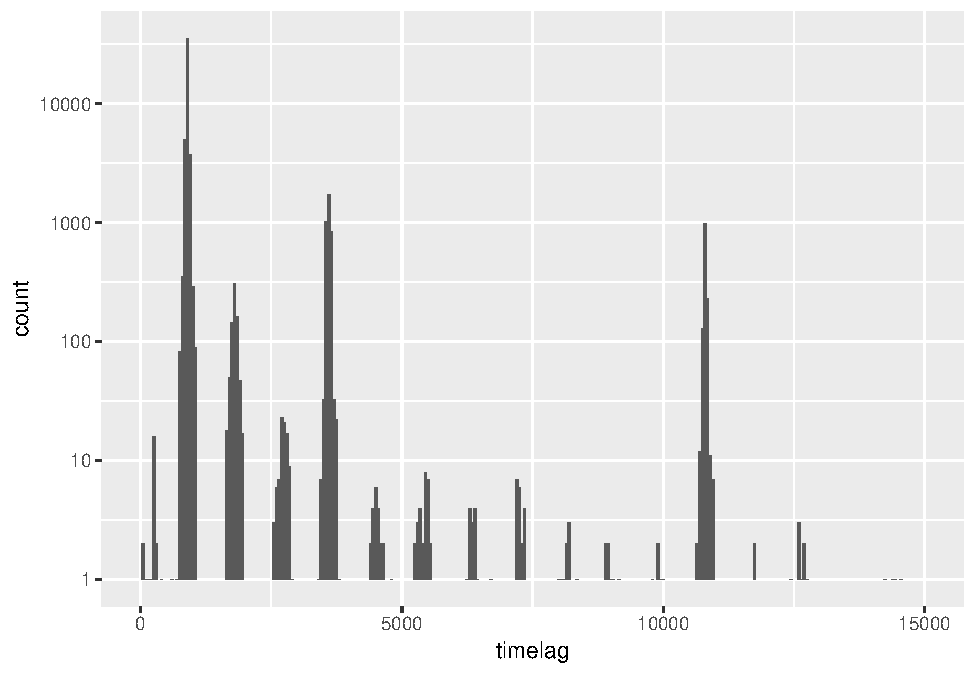
\includegraphics{patterns-and-trends_files/figure-latex/unnamed-chunk-69-2.pdf}
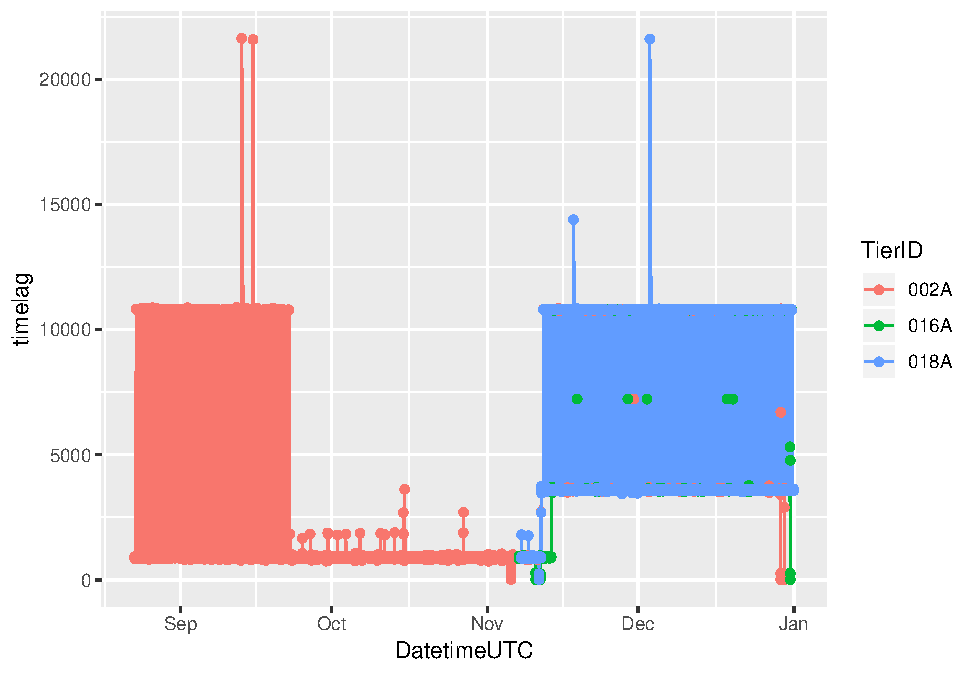
\includegraphics{patterns-and-trends_files/figure-latex/unnamed-chunk-69-3.pdf}

\subsection{Input: Geometry as columns}\label{input-geometry-as-columns}

Last week, we transformed our data from a \texttt{data.frame} to an
\texttt{sf} object. This turned our \texttt{Lat}/\texttt{Long} Columns
into a single geometry (list) column. While this is very handy for many
spatial operations, accessing the coordinates directly becomes
difficult. We therefore suggest storing the information twice, once as a
geometry and once as a numeric value. To do this, we have to extract the
Coordinates using \texttt{st\_coordinates()}. We can store these values
in a new variable and display them:

\begin{Shaded}
\begin{Highlighting}[]
\CommentTok{# Store coordinates in a new variable}

\NormalTok{coordinates <-}\StringTok{ }\KeywordTok{st_coordinates}\NormalTok{(wildschwein_BE)}

\KeywordTok{head}\NormalTok{(coordinates)}
\NormalTok{##         X       Y}
\NormalTok{## 1 2570409 1204752}
\NormalTok{## 2 2570402 1204863}
\NormalTok{## 3 2570394 1204826}
\NormalTok{## 4 2570379 1204817}
\NormalTok{## 5 2570390 1204818}
\NormalTok{## 6 2570390 1204825}
\end{Highlighting}
\end{Shaded}

Note that that the column are named \texttt{X} and \texttt{Y}, while
\href{https://www.swisstopo.admin.ch/de/wissen-fakten/geodaesie-vermessung/neue-koordinaten.html}{\texttt{CH1903+\ LV95}}
names the Axes \texttt{E} and \texttt{N}: let's rename the columns
appropriately. After this, we can use \texttt{cbind()} to ``glue'' the
columns to our original \texttt{sf}-object.

\begin{Shaded}
\begin{Highlighting}[]
\KeywordTok{colnames}\NormalTok{(coordinates) <-}\StringTok{ }\KeywordTok{c}\NormalTok{(}\StringTok{"E"}\NormalTok{,}\StringTok{"N"}\NormalTok{)}

\NormalTok{wildschwein_BE <-}\StringTok{ }\KeywordTok{cbind}\NormalTok{(wildschwein_BE,coordinates)}

\KeywordTok{head}\NormalTok{(wildschwein_BE)}
\NormalTok{## Simple feature collection with 6 features and 7 fields}
\NormalTok{## geometry type:  POINT}
\NormalTok{## dimension:      XY}
\NormalTok{## bbox:           xmin: 2570379 ymin: 1204752 xmax: 2570409 ymax: 1204863}
\NormalTok{## epsg (SRID):    2056}
\NormalTok{## proj4string:    +proj=somerc +lat_0=46.95240555555556 +lon_0=7.439583333333333 +k_0=1 +x_0=2600000 +y_0=1200000 +ellps=bessel +towgs84=674.374,15.056,405.346,0,0,0,0 +units=m +no_defs}
\NormalTok{##   TierID TierName CollarID         DatetimeUTC timelag       E       N}
\NormalTok{## 1   002A     Sabi    12275 2014-08-22 21:00:12     904 2570409 1204752}
\NormalTok{## 2   002A     Sabi    12275 2014-08-22 21:15:16     927 2570402 1204863}
\NormalTok{## 3   002A     Sabi    12275 2014-08-22 21:30:43     924 2570394 1204826}
\NormalTok{## 4   002A     Sabi    12275 2014-08-22 21:46:07     855 2570379 1204817}
\NormalTok{## 5   002A     Sabi    12275 2014-08-22 22:00:22     888 2570390 1204818}
\NormalTok{## 6   002A     Sabi    12275 2014-08-22 22:15:10     903 2570390 1204825}
\NormalTok{##                  geometry}
\NormalTok{## 1 POINT (2570409 1204752)}
\NormalTok{## 2 POINT (2570402 1204863)}
\NormalTok{## 3 POINT (2570394 1204826)}
\NormalTok{## 4 POINT (2570379 1204817)}
\NormalTok{## 5 POINT (2570390 1204818)}
\NormalTok{## 6 POINT (2570390 1204825)}
\end{Highlighting}
\end{Shaded}

\subsection{Task 2: Deriving movement parameters I:
Speed}\label{task-2-deriving-movement-parameters-i-speed}

In this task we will derive some additional movement parameters from our
trajectories. So far our trajectories only consist of a list of
time-stamped spatial locations. So let's calculate the animal's
steplength based on the Euclidean distance between two subsequent
locations.

\begin{itemize}
\tightlist
\item
  You can calculate the Euclidean distance with the following formula:
  \texttt{sqrt((E1-E2)\^{}2+(N1-N2)\^{}2)}
\item
  use \texttt{lead(E,1)} to address the the row \texttt{n+1} (i.e.~E2)
\end{itemize}

Now calculate the animals speed between subsequent locations based on
the steplength as calculated in the previous task and the timelag
between the locations.

\subsection{Task 3: Cross-scale movement
analysis}\label{task-3-cross-scale-movement-analysis}

Laube and Purves (\protect\hyperlink{ref-laube2011}{2011}) analyse
animal movement across different scales (see below). We will do the same
on a \emph{subset} of our data.

\begin{figure}
\centering
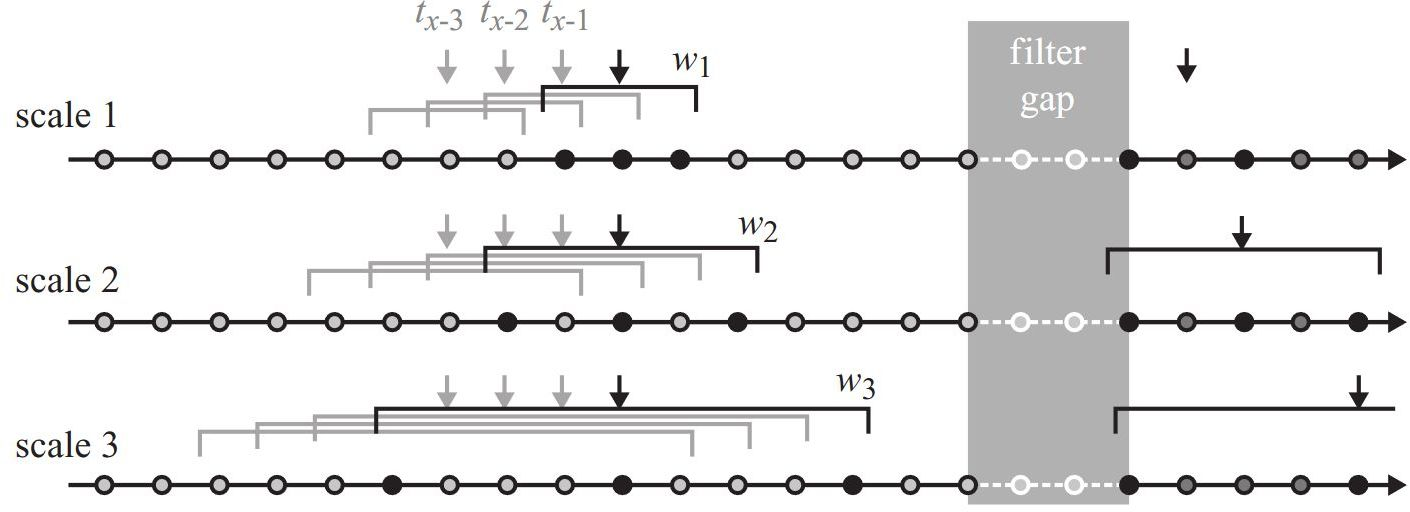
\includegraphics{02_Images/laube_2011_2.jpg}
\caption{Laube and Purves (\protect\hyperlink{ref-laube2011}{2011}):
\emph{Black points are used in calculation of movement parameters
(e.g.~speed) at a given termporal scale.}}
\end{figure}

\subsubsection{\texorpdfstring{Import
``Caro60''}{Import Caro60}}\label{import-caro60}

In the first task, we saw that the animals are sampled at different
frequencies. To simplify the task, we've prepared a dataset that
includes 200 locations of a single wild boar with a constant sampling
interval of 60 seconds. Import this dataset named ``caro60.csv''
(available on moodle) just like you imported the other wild boar data.
\textbf{NOTE:} We've converted the positions to CH1903+ LV95 for your
convenience. Consider this when transforming to \texttt{sf}! Save this
data to a new variable (we will use \texttt{caro60}).

\subsubsection{Resample}\label{resample}

Now manually reduce the granularity of our sampling interval by
selecting every 3\textsuperscript{rd}, 6\textsuperscript{th} and
9\textsuperscript{th} position.

If you like to stick to the \texttt{tidyverse} approach, you can use
\texttt{slice()} to subset the dataset by row number. Slice takes an
integer vector. Eg: \texttt{slice(dataset,\ 1:10)}, returns the first 10
rows of a dataset, \texttt{slice(dataset,\ c(1,5,10))} returns the
1\textsuperscript{st}, 5\textsuperscript{th} and 10\textsuperscript{th}
value of a dataset. Save each re-sampled dataset in a new variable. We
will use \texttt{wildschwein\_BE\_3}, \texttt{wildschwein\_BE\_6} and
\texttt{wildschwein\_BE\_9}.

You should now have 4 data sets with different number of rows:

\begin{Shaded}
\begin{Highlighting}[]
\KeywordTok{nrow}\NormalTok{(caro60)}
\NormalTok{## [1] 200}
\KeywordTok{nrow}\NormalTok{(caro60_}\DecValTok{3}\NormalTok{)}
\NormalTok{## [1] 67}
\KeywordTok{nrow}\NormalTok{(caro60_}\DecValTok{6}\NormalTok{)}
\NormalTok{## [1] 34}
\KeywordTok{nrow}\NormalTok{(caro60_}\DecValTok{9}\NormalTok{)}
\NormalTok{## [1] 23}
\end{Highlighting}
\end{Shaded}

\subsubsection{Update derived
parameters}\label{update-derived-parameters}

\texttt{timelag}, \texttt{steplength} and \texttt{speed} now have to be
recalculated for the three re-sampled data sets. Do so as we illustrated
in the Chapter \emph{Demo}.

\subsubsection{Visualize}\label{visualize}

Compare the speeds in a line plot and visualize the trajectories in a
map (see examples below). Interpret the line plot, what do the different
lines for the different temporal granularities tell you?

We've stored the geographic location of our point in the trajectory in
three different forms in our dataset. Once as a \texttt{geometry}, once
as \texttt{E}/\texttt{N} and once as \texttt{lat}/\texttt{long}. In our
view, it is most practical to use the \texttt{E}/\texttt{N} (integer)
columns of our data to map them in this task

\begin{itemize}
\tightlist
\item
  \texttt{geom\_sf()} does not plot lines, just points
\item
  Therefore, use \texttt{geom\_path()} \emph{and} \texttt{geom\_point()}
  rather than \texttt{geom\_sf()} within \texttt{ggplot}
\item
  In contrast to \texttt{geom\_sf()}, you have to explicitly specify the
  \texttt{x}/\texttt{y} columns (in our case \texttt{E}/\texttt{N}) with
  \texttt{geom\_path()}/\texttt{geom\_point()}
\item
  \texttt{geom\_line()} does not work when mapping trajectory data,
  since it connects the observations \emph{in order of the variable on
  the x axis}. \texttt{geom\_path()} connects the observations in the
  order in which they appear in the data
\end{itemize}

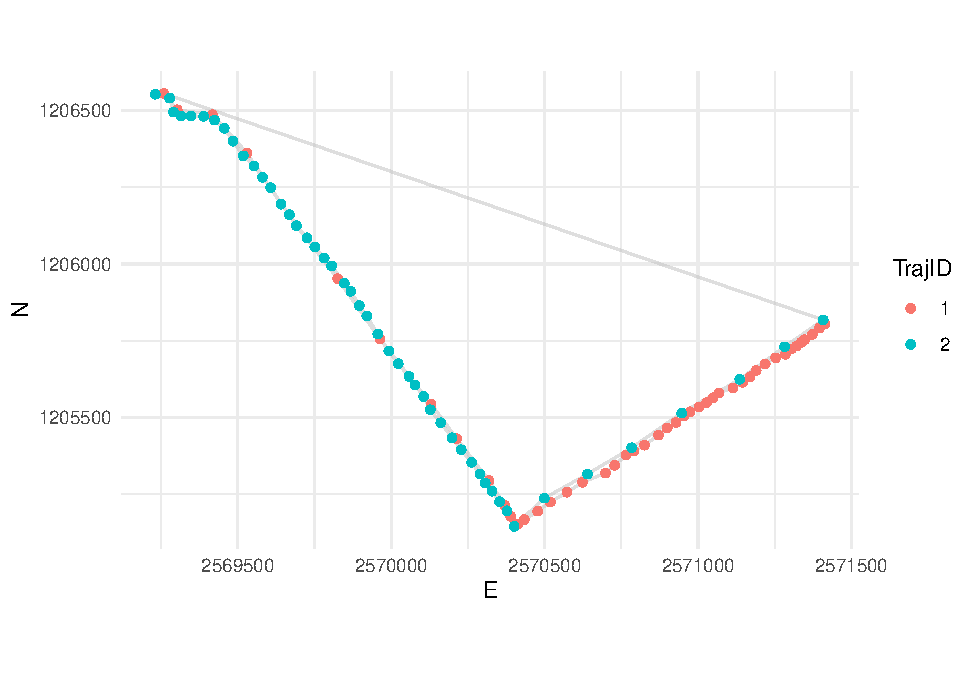
\includegraphics{patterns-and-trends_files/figure-latex/unnamed-chunk-84-1.pdf}
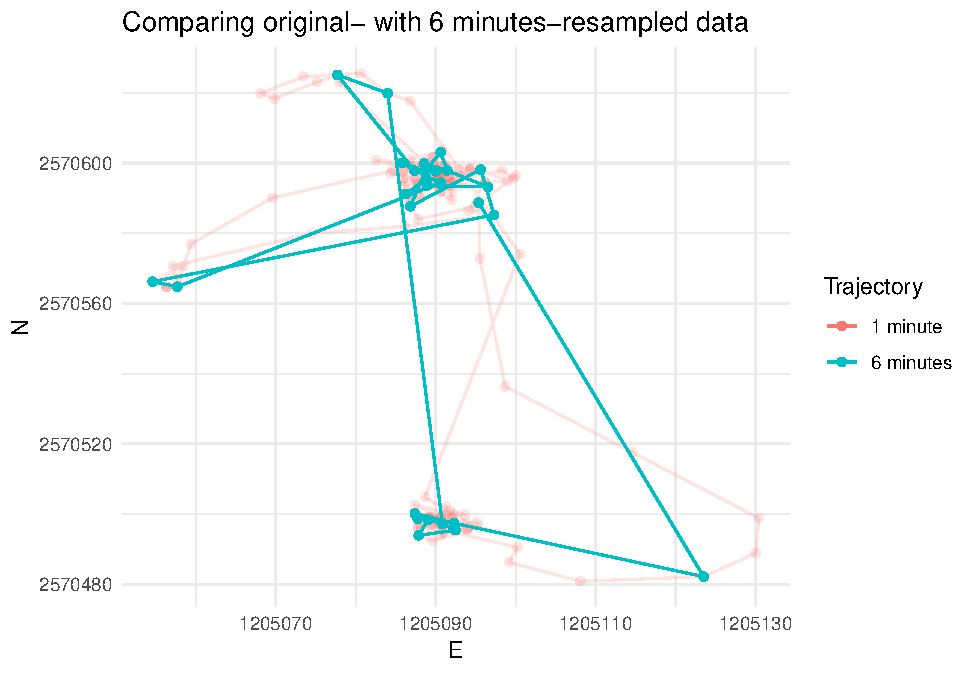
\includegraphics{patterns-and-trends_files/figure-latex/unnamed-chunk-84-2.pdf}
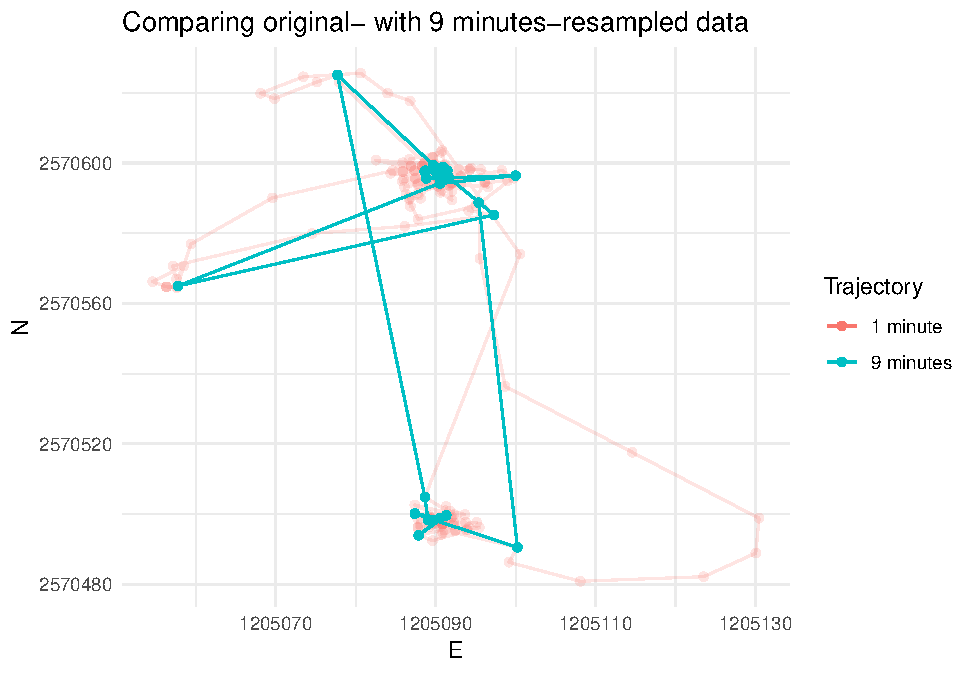
\includegraphics{patterns-and-trends_files/figure-latex/unnamed-chunk-84-3.pdf}
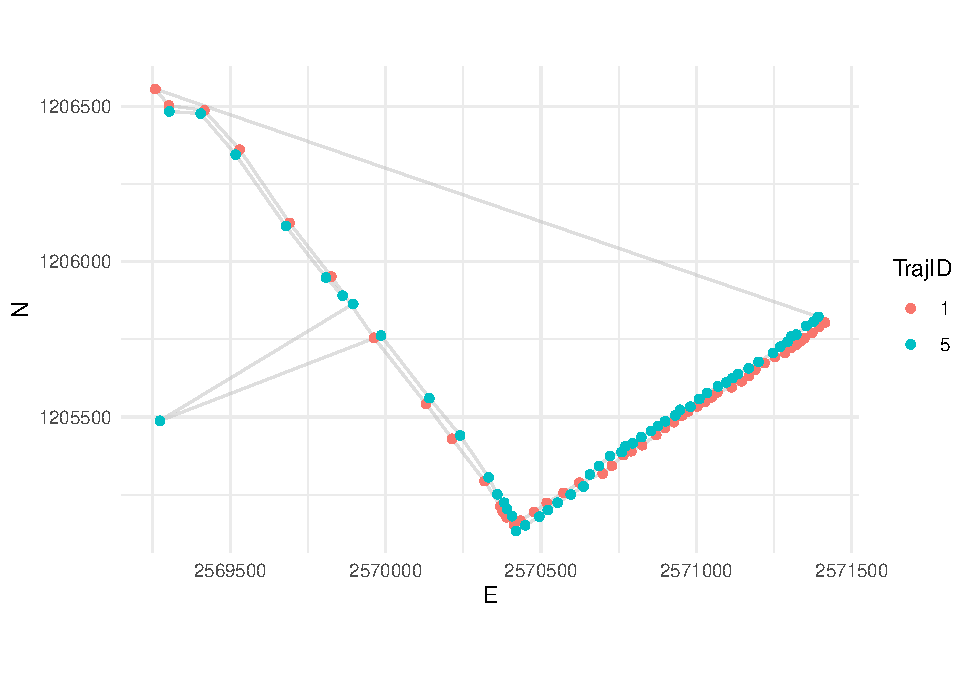
\includegraphics{patterns-and-trends_files/figure-latex/unnamed-chunk-84-4.pdf}

\subsection{Task 4: Deriving movement parameters II: Rolling window
functions}\label{task-4-deriving-movement-parameters-ii-rolling-window-functions}

A different approach would be to \emph{smoothen} the derived parameters
using a
\href{https://docs.wavefront.com/images/5sec_moving_window.png}{moving
window function}. The \texttt{zoo} package offers a variate of moving
window functions (\texttt{roll\_*}). Use \texttt{roll\_mean()} to smooth
the calculated speed. Familiarise yourself with this function by working
on some dummy data, for example:

\begin{Shaded}
\begin{Highlighting}[]

\KeywordTok{library}\NormalTok{(zoo)}

\NormalTok{example <-}\StringTok{ }\KeywordTok{rnorm}\NormalTok{(}\DecValTok{10}\NormalTok{)}
\KeywordTok{rollmean}\NormalTok{(example,}\DataTypeTok{k =} \DecValTok{3}\NormalTok{,}\DataTypeTok{fill =} \OtherTok{NA}\NormalTok{,}\DataTypeTok{align =} \StringTok{"left"}\NormalTok{)}
\NormalTok{##  [1] 0.34583312 0.09405834 0.03823134 0.21921654 0.73911527 0.10131218}
\NormalTok{##  [7] 0.32655714 0.46182911         NA         NA}
\KeywordTok{rollmean}\NormalTok{(example,}\DataTypeTok{k =} \DecValTok{4}\NormalTok{,}\DataTypeTok{fill =} \OtherTok{NA}\NormalTok{,}\DataTypeTok{align =} \StringTok{"left"}\NormalTok{)}
\NormalTok{##  [1] 0.15754877 0.30716897 0.05828676 0.45251038 0.31260935 0.27453111}
\NormalTok{##  [7] 0.63446981         NA         NA         NA}
\end{Highlighting}
\end{Shaded}

Now run \texttt{rollmean}on the \texttt{speed} variable of the subset
(\texttt{wildschwein\_BE\_1}). Visualize the output from your moving
windows and compare different window sizes (\texttt{k\ =}).

\subsection{Task 5 (optional): Calculate turning
angles}\label{task-5-optional-calculate-turning-angles}

Just like we did with \texttt{speed} in tasks 2 - 4, we could do the
same with turning angles of the trajectory. If you like a challenge, try
to calculate these with the same approach! Warning: this task is pretty
complex.

\section{Solutions}\label{solutions}

\subsection{Preperation}\label{preperation-2}

\begin{Shaded}
\begin{Highlighting}[]
\KeywordTok{library}\NormalTok{(tidyverse)}
\KeywordTok{library}\NormalTok{(sf)}
\KeywordTok{library}\NormalTok{(lubridate)}

\NormalTok{wildschwein_BE <-}\StringTok{ }\KeywordTok{read_delim}\NormalTok{(}\StringTok{"00_Rawdata/wildschwein_BE.csv"}\NormalTok{,}\StringTok{","}\NormalTok{)}

\NormalTok{wildschwein_BE =}\StringTok{ }\KeywordTok{st_as_sf}\NormalTok{(wildschwein_BE, }\DataTypeTok{coords =} \KeywordTok{c}\NormalTok{(}\StringTok{"Long"}\NormalTok{, }\StringTok{"Lat"}\NormalTok{), }\DataTypeTok{crs =} \DecValTok{4326}\NormalTok{)}

\NormalTok{wildschwein_BE <-}\StringTok{ }\KeywordTok{st_transform}\NormalTok{(wildschwein_BE, }\DecValTok{2056}\NormalTok{)}
\end{Highlighting}
\end{Shaded}

\subsection{Demo Tidyverse}\label{demo-tidyverse-1}

\begin{Shaded}
\begin{Highlighting}[]
\NormalTok{now <-}\StringTok{ }\KeywordTok{Sys.time}\NormalTok{()}

\NormalTok{later <-}\StringTok{ }\NormalTok{now }\OperatorTok{+}\StringTok{ }\DecValTok{10000}

\NormalTok{time_difference <-}\StringTok{ }\KeywordTok{difftime}\NormalTok{(later,now)}
\NormalTok{time_difference}
\NormalTok{time_difference <-}\StringTok{ }\KeywordTok{difftime}\NormalTok{(later,now,}\DataTypeTok{units =} \StringTok{"mins"}\NormalTok{)}
\NormalTok{time_difference}
\KeywordTok{str}\NormalTok{(time_difference)}
\NormalTok{time_difference <-}\StringTok{ }\KeywordTok{as.numeric}\NormalTok{(}\KeywordTok{difftime}\NormalTok{(later,now,}\DataTypeTok{units =} \StringTok{"mins"}\NormalTok{))}

\KeywordTok{str}\NormalTok{(time_difference)}

\NormalTok{numbers <-}\StringTok{ }\DecValTok{1}\OperatorTok{:}\DecValTok{10}

\NormalTok{numbers}
\KeywordTok{lead}\NormalTok{(numbers)}

\KeywordTok{lead}\NormalTok{(numbers,}\DataTypeTok{n =} \DecValTok{2}\NormalTok{)}

\KeywordTok{lag}\NormalTok{(numbers)}

\KeywordTok{lag}\NormalTok{(numbers,}\DataTypeTok{n =} \DecValTok{5}\NormalTok{)}

\KeywordTok{lag}\NormalTok{(numbers,}\DataTypeTok{n =} \DecValTok{5}\NormalTok{, }\DataTypeTok{default =} \DecValTok{0}\NormalTok{)}
\KeywordTok{lead}\NormalTok{(numbers)}\OperatorTok{-}\NormalTok{numbers}

\NormalTok{wildschwein_BE}\OperatorTok{$}\NormalTok{timelag  <-}\StringTok{ }\KeywordTok{as.numeric}\NormalTok{(}\KeywordTok{difftime}\NormalTok{(}\KeywordTok{lead}\NormalTok{(wildschwein_BE}\OperatorTok{$}\NormalTok{DatetimeUTC),wildschwein_BE}\OperatorTok{$}\NormalTok{DatetimeUTC,}\DataTypeTok{units =} \StringTok{"secs"}\NormalTok{))}

\NormalTok{wildschwein_BE <-}\StringTok{ }\KeywordTok{mutate}\NormalTok{(wildschwein_BE,}\DataTypeTok{timelag =} \KeywordTok{as.numeric}\NormalTok{(}\KeywordTok{difftime}\NormalTok{(}\KeywordTok{lead}\NormalTok{(DatetimeUTC),DatetimeUTC,}\DataTypeTok{units =} \StringTok{"secs"}\NormalTok{)))}
\KeywordTok{summary}\NormalTok{(wildschwein_BE}\OperatorTok{$}\NormalTok{timelag)}
\NormalTok{wildschwein_BE <-}\StringTok{ }\KeywordTok{group_by}\NormalTok{(wildschwein_BE,TierID)}
\NormalTok{wildschwein_BE <-}\StringTok{ }\KeywordTok{mutate}\NormalTok{(wildschwein_BE,}\DataTypeTok{timelag =} \KeywordTok{as.numeric}\NormalTok{(}\KeywordTok{difftime}\NormalTok{(}\KeywordTok{lead}\NormalTok{(DatetimeUTC),DatetimeUTC,}\DataTypeTok{units =} \StringTok{"secs"}\NormalTok{)))}

\KeywordTok{summary}\NormalTok{(wildschwein_BE}\OperatorTok{$}\NormalTok{timelag)}
\NormalTok{## summarise(wildschwein_BE, mean = mean(timelag, na.rm = T))}

\KeywordTok{summarise}\NormalTok{(}\KeywordTok{st_set_geometry}\NormalTok{(wildschwein_BE,}\OtherTok{NULL}\NormalTok{), }\DataTypeTok{mean_timelag =} \KeywordTok{mean}\NormalTok{(timelag, }\DataTypeTok{na.rm =}\NormalTok{ T))}

\NormalTok{wildschwein_BE }\OperatorTok\StringTok{                     }\CommentTok{# Take wildschwein_BE...}
\StringTok{  }\KeywordTok{st_set_geometry}\NormalTok{(}\OtherTok{NULL}\NormalTok{) }\OperatorTok\StringTok{            }\CommentTok{# ...remove the geometry column...}
\StringTok{  }\KeywordTok{group_by}\NormalTok{(TierID) }\OperatorTok\StringTok{                 }\CommentTok{# ...group it by TierID}
\StringTok{  }\KeywordTok{summarise}\NormalTok{(                           }\CommentTok{# Summarise the data...}
    \DataTypeTok{mean_timelag =} \KeywordTok{mean}\NormalTok{(timelag,}\DataTypeTok{na.rm =}\NormalTok{ T) }\CommentTok{# ...by calculating the mean timelag}
\NormalTok{  )}
\NormalTok{pigs =}\StringTok{ }\KeywordTok{data.frame}\NormalTok{(}
  \DataTypeTok{TierID=}\KeywordTok{c}\NormalTok{(}\DecValTok{8001}\NormalTok{,}\DecValTok{8003}\NormalTok{,}\DecValTok{8004}\NormalTok{,}\DecValTok{8005}\NormalTok{,}\DecValTok{8800}\NormalTok{,}\DecValTok{8820}\NormalTok{,}\DecValTok{3000}\NormalTok{,}\DecValTok{3001}\NormalTok{,}\DecValTok{3002}\NormalTok{,}\DecValTok{3003}\NormalTok{,}\DecValTok{8330}\NormalTok{,}\DecValTok{7222}\NormalTok{),}
  \DataTypeTok{sex=}\KeywordTok{c}\NormalTok{(}\StringTok{"M"}\NormalTok{,}\StringTok{"M"}\NormalTok{,}\StringTok{"M"}\NormalTok{,}\StringTok{"F"}\NormalTok{,}\StringTok{"M"}\NormalTok{,}\StringTok{"M"}\NormalTok{,}\StringTok{"F"}\NormalTok{,}\StringTok{"F"}\NormalTok{,}\StringTok{"M"}\NormalTok{,}\StringTok{"F"}\NormalTok{,}\StringTok{"M"}\NormalTok{,}\StringTok{"F"}\NormalTok{),}
  \DataTypeTok{age=}\KeywordTok{c}\NormalTok{(}\StringTok{"A"}\NormalTok{,}\StringTok{"A"}\NormalTok{,}\StringTok{"J"}\NormalTok{,}\StringTok{"A"}\NormalTok{,}\StringTok{"J"}\NormalTok{,}\StringTok{"J"}\NormalTok{,}\StringTok{"J"}\NormalTok{,}\StringTok{"A"}\NormalTok{,}\StringTok{"J"}\NormalTok{,}\StringTok{"J"}\NormalTok{,}\StringTok{"A"}\NormalTok{,}\StringTok{"A"}\NormalTok{),}
  \DataTypeTok{weight=}\KeywordTok{c}\NormalTok{(}\FloatTok{50.755}\NormalTok{,}\FloatTok{43.409}\NormalTok{,}\FloatTok{12.000}\NormalTok{,}\FloatTok{16.787}\NormalTok{,}\FloatTok{20.987}\NormalTok{,}\FloatTok{25.765}\NormalTok{,}\FloatTok{22.0122}\NormalTok{,}\FloatTok{21.343}\NormalTok{,}\FloatTok{12.532}\NormalTok{,}\FloatTok{54.32}\NormalTok{,}\FloatTok{11.027}\NormalTok{,}\FloatTok{88.08}\NormalTok{)}
\NormalTok{)}

\NormalTok{pigs}

\NormalTok{pigs }\OperatorTok
\StringTok{    }\KeywordTok{summarise}\NormalTok{(         }
    \DataTypeTok{mean_weight =} \KeywordTok{mean}\NormalTok{(weight)}
\NormalTok{  )}

\NormalTok{pigs }\OperatorTok
\StringTok{  }\KeywordTok{group_by}\NormalTok{(sex) }\OperatorTok
\StringTok{  }\KeywordTok{summarise}\NormalTok{(         }
    \DataTypeTok{mean_weight =} \KeywordTok{mean}\NormalTok{(weight)}
\NormalTok{  )}

\NormalTok{pigs }\OperatorTok
\StringTok{  }\KeywordTok{group_by}\NormalTok{(sex,age) }\OperatorTok
\StringTok{  }\KeywordTok{summarise}\NormalTok{(         }
    \DataTypeTok{mean_weight =} \KeywordTok{mean}\NormalTok{(weight)}
\NormalTok{  )}
\end{Highlighting}
\end{Shaded}

\subsection{Task 1}\label{task-1}

\begin{Shaded}
\begin{Highlighting}[]

\NormalTok{wildschwein_BE <-}\StringTok{ }\NormalTok{wildschwein_BE }\OperatorTok
\StringTok{  }\KeywordTok{mutate}\NormalTok{(}\DataTypeTok{timelag =} \KeywordTok{as.numeric}\NormalTok{(}\KeywordTok{difftime}\NormalTok{(}\KeywordTok{lead}\NormalTok{(DatetimeUTC),DatetimeUTC,}\DataTypeTok{units =} \StringTok{"secs"}\NormalTok{)))}

\KeywordTok{ggplot}\NormalTok{(wildschwein_BE, }\KeywordTok{aes}\NormalTok{(DatetimeUTC,TierID)) }\OperatorTok{+}
\StringTok{  }\KeywordTok{geom_line}\NormalTok{()}

\KeywordTok{ggplot}\NormalTok{(wildschwein_BE, }\KeywordTok{aes}\NormalTok{(timelag)) }\OperatorTok{+}
\StringTok{  }\KeywordTok{geom_histogram}\NormalTok{(}\DataTypeTok{binwidth =} \DecValTok{50}\NormalTok{) }\OperatorTok{+}
\StringTok{  }\KeywordTok{lims}\NormalTok{(}\DataTypeTok{x =} \KeywordTok{c}\NormalTok{(}\DecValTok{0}\NormalTok{,}\DecValTok{15000}\NormalTok{)) }\OperatorTok{+}
\StringTok{  }\KeywordTok{scale_y_log10}\NormalTok{()}
  

\NormalTok{wildschwein_BE }\OperatorTok
\StringTok{  }\KeywordTok{filter}\NormalTok{(}\KeywordTok{year}\NormalTok{(DatetimeUTC)  }\OperatorTok{==}\StringTok{ }\DecValTok{2014}\NormalTok{) }\OperatorTok
\StringTok{  }\KeywordTok{ggplot}\NormalTok{(}\KeywordTok{aes}\NormalTok{(DatetimeUTC,timelag, }\DataTypeTok{colour =}\NormalTok{ TierID)) }\OperatorTok{+}
\StringTok{  }\KeywordTok{geom_line}\NormalTok{() }\OperatorTok{+}
\StringTok{  }\KeywordTok{geom_point}\NormalTok{()}
  
\end{Highlighting}
\end{Shaded}

\subsection{Input}\label{input}

\begin{Shaded}
\begin{Highlighting}[]
\CommentTok{# Store coordinates in a new variable}

\NormalTok{coordinates <-}\StringTok{ }\KeywordTok{st_coordinates}\NormalTok{(wildschwein_BE)}

\KeywordTok{head}\NormalTok{(coordinates)}
\KeywordTok{colnames}\NormalTok{(coordinates) <-}\StringTok{ }\KeywordTok{c}\NormalTok{(}\StringTok{"E"}\NormalTok{,}\StringTok{"N"}\NormalTok{)}

\NormalTok{wildschwein_BE <-}\StringTok{ }\KeywordTok{cbind}\NormalTok{(wildschwein_BE,coordinates)}

\KeywordTok{head}\NormalTok{(wildschwein_BE)}
\end{Highlighting}
\end{Shaded}

\subsection{Task 2}\label{task-2}

\begin{Shaded}
\begin{Highlighting}[]

\NormalTok{wildschwein_BE <-}\StringTok{ }\NormalTok{wildschwein_BE }\OperatorTok
\StringTok{  }\KeywordTok{group_by}\NormalTok{(TierID) }\OperatorTok
\StringTok{  }\KeywordTok{mutate}\NormalTok{(}
    \DataTypeTok{steplength =} \KeywordTok{sqrt}\NormalTok{((E}\OperatorTok{-}\KeywordTok{lead}\NormalTok{(E))}\OperatorTok{^}\DecValTok{2}\OperatorTok{+}\NormalTok{(N}\OperatorTok{-}\KeywordTok{lead}\NormalTok{(N))}\OperatorTok{^}\DecValTok{2}\NormalTok{)}
\NormalTok{  )}
\NormalTok{wildschwein_BE <-}\StringTok{ }\NormalTok{wildschwein_BE }\OperatorTok
\StringTok{  }\KeywordTok{group_by}\NormalTok{(TierID) }\OperatorTok
\StringTok{  }\KeywordTok{mutate}\NormalTok{(}
    \DataTypeTok{speed =}\NormalTok{ steplength}\OperatorTok{/}\NormalTok{timelag}
\NormalTok{  )}
\end{Highlighting}
\end{Shaded}

\subsection{Task 3}\label{task-3}

\begin{Shaded}
\begin{Highlighting}[]
\NormalTok{caro60 <-}\StringTok{ }\KeywordTok{read_delim}\NormalTok{(}\StringTok{"00_Rawdata/caro60.csv"}\NormalTok{,}\StringTok{","}\NormalTok{) }\OperatorTok
\StringTok{  }\KeywordTok{st_as_sf}\NormalTok{(}\DataTypeTok{coords =} \KeywordTok{c}\NormalTok{(}\StringTok{"E"}\NormalTok{, }\StringTok{"N"}\NormalTok{), }\DataTypeTok{crs =} \DecValTok{2056}\NormalTok{, }\DataTypeTok{remove =} \OtherTok{FALSE}\NormalTok{)}
  
\NormalTok{caro60_}\DecValTok{3}\NormalTok{ <-}\StringTok{ }\NormalTok{caro60 }\OperatorTok
\StringTok{  }\KeywordTok{slice}\NormalTok{(}\KeywordTok{seq}\NormalTok{(}\DecValTok{1}\NormalTok{,}\KeywordTok{nrow}\NormalTok{(.),}\DecValTok{3}\NormalTok{)) }\CommentTok{# the dot (".") represents the piped dataset}

\NormalTok{caro60_}\DecValTok{6}\NormalTok{ <-}\StringTok{ }\NormalTok{caro60 }\OperatorTok
\StringTok{  }\KeywordTok{slice}\NormalTok{(}\KeywordTok{seq}\NormalTok{(}\DecValTok{1}\NormalTok{,}\KeywordTok{nrow}\NormalTok{(.),}\DecValTok{6}\NormalTok{))}

\NormalTok{caro60_}\DecValTok{9}\NormalTok{ <-}\StringTok{ }\NormalTok{caro60 }\OperatorTok
\StringTok{  }\KeywordTok{slice}\NormalTok{(}\KeywordTok{seq}\NormalTok{(}\DecValTok{1}\NormalTok{,}\KeywordTok{nrow}\NormalTok{(.),}\DecValTok{9}\NormalTok{))}
\KeywordTok{nrow}\NormalTok{(caro60)}
\KeywordTok{nrow}\NormalTok{(caro60_}\DecValTok{3}\NormalTok{)}
\KeywordTok{nrow}\NormalTok{(caro60_}\DecValTok{6}\NormalTok{)}
\KeywordTok{nrow}\NormalTok{(caro60_}\DecValTok{9}\NormalTok{)}

\NormalTok{caro60 <-}\StringTok{ }\NormalTok{caro60 }\OperatorTok
\StringTok{  }\KeywordTok{mutate}\NormalTok{(}
    \DataTypeTok{timelag =} \KeywordTok{as.numeric}\NormalTok{(}\KeywordTok{difftime}\NormalTok{(}\KeywordTok{lead}\NormalTok{(DatetimeUTC),DatetimeUTC,}\DataTypeTok{units =} \StringTok{"secs"}\NormalTok{)),}
    \DataTypeTok{steplength =} \KeywordTok{sqrt}\NormalTok{((E}\OperatorTok{-}\KeywordTok{lead}\NormalTok{(E))}\OperatorTok{^}\DecValTok{2}\OperatorTok{+}\NormalTok{(N}\OperatorTok{-}\KeywordTok{lead}\NormalTok{(N))}\OperatorTok{^}\DecValTok{2}\NormalTok{),}
    \DataTypeTok{speed =}\NormalTok{ steplength}\OperatorTok{/}\NormalTok{timelag}
\NormalTok{  )}

\NormalTok{caro60_}\DecValTok{3}\NormalTok{ <-}\StringTok{ }\NormalTok{caro60_}\DecValTok{3} \OperatorTok
\StringTok{  }\KeywordTok{mutate}\NormalTok{(}
    \DataTypeTok{timelag =} \KeywordTok{as.numeric}\NormalTok{(}\KeywordTok{difftime}\NormalTok{(}\KeywordTok{lead}\NormalTok{(DatetimeUTC),DatetimeUTC,}\DataTypeTok{units =} \StringTok{"secs"}\NormalTok{)),}
    \DataTypeTok{steplength =} \KeywordTok{sqrt}\NormalTok{((E}\OperatorTok{-}\KeywordTok{lead}\NormalTok{(E))}\OperatorTok{^}\DecValTok{2}\OperatorTok{+}\NormalTok{(N}\OperatorTok{-}\KeywordTok{lead}\NormalTok{(N))}\OperatorTok{^}\DecValTok{2}\NormalTok{),}
    \DataTypeTok{speed =}\NormalTok{ steplength}\OperatorTok{/}\NormalTok{timelag}
\NormalTok{  )}

\NormalTok{caro60_}\DecValTok{6}\NormalTok{ <-}\StringTok{ }\NormalTok{caro60_}\DecValTok{6} \OperatorTok
\StringTok{  }\KeywordTok{mutate}\NormalTok{(}
    \DataTypeTok{timelag =} \KeywordTok{as.numeric}\NormalTok{(}\KeywordTok{difftime}\NormalTok{(}\KeywordTok{lead}\NormalTok{(DatetimeUTC),DatetimeUTC,}\DataTypeTok{units =} \StringTok{"secs"}\NormalTok{)),}
    \DataTypeTok{steplength =} \KeywordTok{sqrt}\NormalTok{((E}\OperatorTok{-}\KeywordTok{lead}\NormalTok{(E))}\OperatorTok{^}\DecValTok{2}\OperatorTok{+}\NormalTok{(N}\OperatorTok{-}\KeywordTok{lead}\NormalTok{(N))}\OperatorTok{^}\DecValTok{2}\NormalTok{),}
    \DataTypeTok{speed =}\NormalTok{ steplength}\OperatorTok{/}\NormalTok{timelag}
\NormalTok{  )}


\NormalTok{caro60_}\DecValTok{9}\NormalTok{ <-}\StringTok{ }\NormalTok{caro60_}\DecValTok{9} \OperatorTok
\StringTok{  }\KeywordTok{mutate}\NormalTok{(}
    \DataTypeTok{timelag =} \KeywordTok{as.numeric}\NormalTok{(}\KeywordTok{difftime}\NormalTok{(}\KeywordTok{lead}\NormalTok{(DatetimeUTC),DatetimeUTC,}\DataTypeTok{units =} \StringTok{"secs"}\NormalTok{)),}
    \DataTypeTok{steplength =} \KeywordTok{sqrt}\NormalTok{((E}\OperatorTok{-}\KeywordTok{lead}\NormalTok{(E))}\OperatorTok{^}\DecValTok{2}\OperatorTok{+}\NormalTok{(N}\OperatorTok{-}\KeywordTok{lead}\NormalTok{(N))}\OperatorTok{^}\DecValTok{2}\NormalTok{),}
    \DataTypeTok{speed =}\NormalTok{ steplength}\OperatorTok{/}\NormalTok{timelag}
\NormalTok{  )}




\KeywordTok{ggplot}\NormalTok{() }\OperatorTok{+}
\StringTok{  }\KeywordTok{geom_point}\NormalTok{(}\DataTypeTok{data =}\NormalTok{ caro60, }\KeywordTok{aes}\NormalTok{(E,N, }\DataTypeTok{colour =} \StringTok{"1 minute"}\NormalTok{), }\DataTypeTok{alpha =} \FloatTok{0.2}\NormalTok{) }\OperatorTok{+}
\StringTok{  }\KeywordTok{geom_path}\NormalTok{(}\DataTypeTok{data =}\NormalTok{ caro60, }\KeywordTok{aes}\NormalTok{(E,N, }\DataTypeTok{colour =} \StringTok{"1 minute"}\NormalTok{), }\DataTypeTok{alpha =} \FloatTok{0.2}\NormalTok{) }\OperatorTok{+}
\StringTok{  }\KeywordTok{geom_point}\NormalTok{(}\DataTypeTok{data =}\NormalTok{ caro60_}\DecValTok{3}\NormalTok{, }\KeywordTok{aes}\NormalTok{(E,N, }\DataTypeTok{colour =} \StringTok{"3 minutes"}\NormalTok{)) }\OperatorTok{+}
\StringTok{  }\KeywordTok{geom_path}\NormalTok{(}\DataTypeTok{data =}\NormalTok{ caro60_}\DecValTok{3}\NormalTok{, }\KeywordTok{aes}\NormalTok{(E,N, }\DataTypeTok{colour =} \StringTok{"3 minutes"}\NormalTok{)) }\OperatorTok{+}
\StringTok{  }\KeywordTok{labs}\NormalTok{(}\DataTypeTok{color=}\StringTok{"Trajectory"}\NormalTok{, }\DataTypeTok{title =} \StringTok{"Comparing original- with 3 minutes-resampled data"}\NormalTok{)  }\OperatorTok{+}
\StringTok{  }\KeywordTok{theme_minimal}\NormalTok{()}

\KeywordTok{ggplot}\NormalTok{() }\OperatorTok{+}
\StringTok{  }\KeywordTok{geom_point}\NormalTok{(}\DataTypeTok{data =}\NormalTok{ caro60, }\KeywordTok{aes}\NormalTok{(E,N, }\DataTypeTok{colour =} \StringTok{"1 minute"}\NormalTok{), }\DataTypeTok{alpha =} \FloatTok{0.2}\NormalTok{) }\OperatorTok{+}
\StringTok{  }\KeywordTok{geom_path}\NormalTok{(}\DataTypeTok{data =}\NormalTok{ caro60, }\KeywordTok{aes}\NormalTok{(E,N, }\DataTypeTok{colour =} \StringTok{"1 minute"}\NormalTok{), }\DataTypeTok{alpha =} \FloatTok{0.2}\NormalTok{) }\OperatorTok{+}
\StringTok{  }\KeywordTok{geom_point}\NormalTok{(}\DataTypeTok{data =}\NormalTok{ caro60_}\DecValTok{6}\NormalTok{, }\KeywordTok{aes}\NormalTok{(E,N, }\DataTypeTok{colour =} \StringTok{"6 minutes"}\NormalTok{)) }\OperatorTok{+}
\StringTok{  }\KeywordTok{geom_path}\NormalTok{(}\DataTypeTok{data =}\NormalTok{ caro60_}\DecValTok{6}\NormalTok{, }\KeywordTok{aes}\NormalTok{(E,N, }\DataTypeTok{colour =} \StringTok{"6 minutes"}\NormalTok{)) }\OperatorTok{+}
\StringTok{  }\KeywordTok{labs}\NormalTok{(}\DataTypeTok{color=}\StringTok{"Trajectory"}\NormalTok{, }\DataTypeTok{title =} \StringTok{"Comparing original- with 6 minutes-resampled data"}\NormalTok{) }\OperatorTok{+}
\StringTok{  }\KeywordTok{theme_minimal}\NormalTok{()}

\KeywordTok{ggplot}\NormalTok{() }\OperatorTok{+}
\StringTok{  }\KeywordTok{geom_point}\NormalTok{(}\DataTypeTok{data =}\NormalTok{ caro60, }\KeywordTok{aes}\NormalTok{(E,N, }\DataTypeTok{colour =} \StringTok{"1 minute"}\NormalTok{), }\DataTypeTok{alpha =} \FloatTok{0.2}\NormalTok{) }\OperatorTok{+}
\StringTok{  }\KeywordTok{geom_path}\NormalTok{(}\DataTypeTok{data =}\NormalTok{ caro60, }\KeywordTok{aes}\NormalTok{(E,N, }\DataTypeTok{colour =} \StringTok{"1 minute"}\NormalTok{), }\DataTypeTok{alpha =} \FloatTok{0.2}\NormalTok{) }\OperatorTok{+}
\StringTok{  }\KeywordTok{geom_point}\NormalTok{(}\DataTypeTok{data =}\NormalTok{ caro60_}\DecValTok{9}\NormalTok{, }\KeywordTok{aes}\NormalTok{(E,N, }\DataTypeTok{colour =} \StringTok{"9 minutes"}\NormalTok{)) }\OperatorTok{+}
\StringTok{  }\KeywordTok{geom_path}\NormalTok{(}\DataTypeTok{data =}\NormalTok{ caro60_}\DecValTok{9}\NormalTok{, }\KeywordTok{aes}\NormalTok{(E,N, }\DataTypeTok{colour =} \StringTok{"9 minutes"}\NormalTok{))}\OperatorTok{+}
\StringTok{  }\KeywordTok{labs}\NormalTok{(}\DataTypeTok{color=}\StringTok{"Trajectory"}\NormalTok{, }\DataTypeTok{title =} \StringTok{"Comparing original- with 9 minutes-resampled data"}\NormalTok{) }\OperatorTok{+}
\StringTok{  }\KeywordTok{theme_minimal}\NormalTok{()}


\KeywordTok{ggplot}\NormalTok{() }\OperatorTok{+}
\StringTok{  }\KeywordTok{geom_line}\NormalTok{(}\DataTypeTok{data =}\NormalTok{ caro60, }\KeywordTok{aes}\NormalTok{(DatetimeUTC,speed, }\DataTypeTok{colour =} \StringTok{"1 minute"}\NormalTok{)) }\OperatorTok{+}
\StringTok{  }\KeywordTok{geom_line}\NormalTok{(}\DataTypeTok{data =}\NormalTok{ caro60_}\DecValTok{3}\NormalTok{, }\KeywordTok{aes}\NormalTok{(DatetimeUTC,speed, }\DataTypeTok{colour =} \StringTok{"3 minutes"}\NormalTok{)) }\OperatorTok{+}
\StringTok{  }\KeywordTok{geom_line}\NormalTok{(}\DataTypeTok{data =}\NormalTok{ caro60_}\DecValTok{6}\NormalTok{, }\KeywordTok{aes}\NormalTok{(DatetimeUTC,speed, }\DataTypeTok{colour =} \StringTok{"6 minutes"}\NormalTok{)) }\OperatorTok{+}
\StringTok{  }\KeywordTok{geom_line}\NormalTok{(}\DataTypeTok{data =}\NormalTok{ caro60_}\DecValTok{9}\NormalTok{, }\KeywordTok{aes}\NormalTok{(DatetimeUTC,speed, }\DataTypeTok{colour =} \StringTok{"9 minutes"}\NormalTok{)) }\OperatorTok{+}
\StringTok{  }\KeywordTok{labs}\NormalTok{(}\DataTypeTok{x =} \StringTok{"Time"}\NormalTok{,}\DataTypeTok{y =} \StringTok{"Speed (m/s)"}\NormalTok{, }\DataTypeTok{title =} \StringTok{"Comparing derived speed at different sampling intervals"}\NormalTok{) }\OperatorTok{+}
\StringTok{  }\KeywordTok{theme_minimal}\NormalTok{()}
\end{Highlighting}
\end{Shaded}

\subsection{Task 4}\label{task-4}

\begin{Shaded}
\begin{Highlighting}[]

\KeywordTok{library}\NormalTok{(zoo)}

\NormalTok{example <-}\StringTok{ }\KeywordTok{rnorm}\NormalTok{(}\DecValTok{10}\NormalTok{)}
\KeywordTok{rollmean}\NormalTok{(example,}\DataTypeTok{k =} \DecValTok{3}\NormalTok{,}\DataTypeTok{fill =} \OtherTok{NA}\NormalTok{,}\DataTypeTok{align =} \StringTok{"left"}\NormalTok{)}
\KeywordTok{rollmean}\NormalTok{(example,}\DataTypeTok{k =} \DecValTok{4}\NormalTok{,}\DataTypeTok{fill =} \OtherTok{NA}\NormalTok{,}\DataTypeTok{align =} \StringTok{"left"}\NormalTok{)}


\NormalTok{caro60 <-}\StringTok{ }\NormalTok{caro60 }\OperatorTok
\StringTok{  }\KeywordTok{mutate}\NormalTok{(}
    \DataTypeTok{speed3 =} \KeywordTok{rollmean}\NormalTok{(speed,}\DecValTok{3}\NormalTok{,}\OtherTok{NA}\NormalTok{,}\DataTypeTok{align =} \StringTok{"left"}\NormalTok{),}
    \DataTypeTok{speed6 =} \KeywordTok{rollmean}\NormalTok{(speed,}\DecValTok{6}\NormalTok{,}\OtherTok{NA}\NormalTok{,}\DataTypeTok{align =} \StringTok{"left"}\NormalTok{),}
    \DataTypeTok{speed9 =} \KeywordTok{rollmean}\NormalTok{(speed,}\DecValTok{9}\NormalTok{,}\OtherTok{NA}\NormalTok{,}\DataTypeTok{align =} \StringTok{"left"}\NormalTok{)}
\NormalTok{  )}

\NormalTok{caro60 }\OperatorTok
\StringTok{  }\KeywordTok{gather}\NormalTok{(key,val,}\KeywordTok{c}\NormalTok{(speed,speed3,speed6,speed9)) }\OperatorTok
\StringTok{  }\KeywordTok{ggplot}\NormalTok{(}\KeywordTok{aes}\NormalTok{(DatetimeUTC,val,}\DataTypeTok{colour =}\NormalTok{ key,}\DataTypeTok{group =}\NormalTok{ key)) }\OperatorTok{+}
\StringTok{  }\CommentTok{# geom_point() +}
\StringTok{  }\KeywordTok{geom_line}\NormalTok{() }
\end{Highlighting}
\end{Shaded}

\subsection{Task 5}\label{task-5}

\chapter*{References}\label{references}
\addcontentsline{toc}{chapter}{References}

\hypertarget{refs}{}
\hypertarget{ref-laube2011}{}
Laube, Patrick, and Ross S. Purves. 2011. ``How Fast Is a Cow? Cross -
Scale Analysis of Movement Data.'' \emph{Transactions in GIS} 15 (3):
401--18.
doi:\href{https://doi.org/10.1111/j.1467-9671.2011.01256.x}{10.1111/j.1467-9671.2011.01256.x}.

\hypertarget{ref-wickham2017}{}
Wickham, Hadley, and Garrett Grolemund. 2017. \emph{R for Data Science:
Import, Tidy, Transform, Visualize, and Model Data}. 1st ed. O'Reilly
Media, Inc.


\end{document}
